\documentclass[a4paper,11pt]{article}
\usepackage{graphicx}
\usepackage{amssymb, amsmath}
\usepackage{subcaption}
\usepackage{float}
\usepackage{setspace}
\usepackage{siunitx}
\usepackage{sectsty}
\allsectionsfont{\centering}

\usepackage{natbib}
\usepackage{booktabs} 
\usepackage{mathrsfs}
\usepackage[section]{placeins} % use the command \FloatBarrier to keep figures from migrating too far

\usepackage{titlesec} % for changing formatting of sections
\titleformat{\section}{\normalfont\huge\scshape\raggedright}{\thesection}{1em}{} 
%\raggedright gets rid of hyphenation in section titles
\titleformat{\subsection}{\normalfont\Large\raggedright}{\thesubsection}{1em}{}
\titleformat{\subsubsection}{\normalfont\normalsize\itshape}{\thesubsubsection}{1em}{}

\usepackage{indentfirst} % include to indent the first paragraphs after a section 

\usepackage[top=1.5in, bottom=1.5in, left=1.5in, right=1in]{geometry}
\usepackage[font=footnotesize,labelfont=bf,skip=2pt]{caption}
% set section number fonts
%\usepackage{titlesec}
%%\titleformat{\subsection}
%  %{\normalfont\fontsize{10.95}{15}\bfseries}{\thesection}{1em}{}
%\titleformat{\subsection}
%  {\normalfont\fontsize{11}{5}\bfseries}{\thesubsection}{1em}{}
%	\titleformat{\subsubsection}
%  {\normalfont\fontsize{10}{3}\bfseries}{\thesubsubsection}{1em}{}

\setlength{\headheight}{14pt} 

% fancy header and footer
\usepackage{fancyhdr}
\pagestyle{fancy}
\fancyhf{}
\fancyhead[R]{\leftmark}
\fancyfoot[R]{\thepage}

\renewcommand\subsectionmark[1]{\markboth{\itshape\MakeUppercase{#1}}{}}
\renewcommand{\footrulewidth}{0pt}

\usepackage[bookmarks=true,hidelinks]{hyperref}

%%%%%%%%%%%%%%%%%%%%%%%%%%
%  My Commands
%%%%%%%%%%%%%%%%%%%%%%%%%%

\def\d{\mathrm{d}}
\def\L{\mathscr{L}}
\def\half{\tfrac{1}{2}}
\def\nsr{$n_s$-$r$ }

\usepackage{color}
\definecolor{applegreen}{rgb}{0.55, 0.71, 0.0}
\newcommand{\mep}[1]{{\color{applegreen} \textbf{[MEP:  #1]}}}
\newcommand{\hl}[1]{\colorbox{yellow}{#1}}



\begin{document}

\begin{titlepage}

\newcommand{\HRule}{\rule{\linewidth}{0.5mm}} % Defines a new command for the horizontal lines, change thickness here
%----------------------------------------------------------------------------------------
%	LOGO SECTION
%----------------------------------------------------------------------------------------

%\noindent
%\raisebox{-1.5\height}{\includegraphics[width=0.47\textwidth]{IMSB_LongLogo.png}} \\[2cm]
\begin{centering}
\textsc{\huge Princeton University}\\
\textsc{\Large Department of Astrophysical Sciences}\\[2cm]
\end{centering}
%----------------------------------------------------------------------------------------
\center % Center everything on the page
%----------------------------------------------------------------------------------------
%	HEADING SECTIONS
%----------------------------------------------------------------------------------------

%\textsc{\LARGE ETH Z\"urich}\\[1.5cm] % Name of your university/college
%\textsc{\Large Institute of Molecular Systems Biology}\\[0.5cm] % Major heading such as course name

%----------------------------------------------------------------------------------------
%	TITLE SECTION
%----------------------------------------------------------------------------------------

\HRule \\[0.4cm]
{\LARGE \bfseries Quantifying the Degree of Fine-tuning in Models of Inflation}\\[0.4cm] % Title of your document
\HRule \\[1cm]

\textsc{\Large Senior Thesis}\\[0cm] % Minor heading such as course title

%----------------------------------------------------------------------------------------
%	DATE SECTION
%----------------------------------------------------------------------------------------
\textsc{\Large 2015}\\[2cm] % Date, change the \today to a set date if you want to be precise

\includegraphics[width=0.35\textwidth]{figures/PrincetonShield.pdf}\\[2cm]

%----------------------------------------------------------------------------------------
%	AUTHOR SECTION
%----------------------------------------------------------------------------------------
\hfill
\begin{minipage}{0.5\textwidth}
\begin{flushright} \Large
\emph{Author:}\\
Morgan Presley\\[1cm] % Your name
\emph{Adviser:} \\
Professor Paul Steinhardt\\[0.5cm]
%\emph{Second Reader:} \\
%Professor David \textsc{Spergel}
\end{flushright}
\end{minipage}\\[4cm]

\vfill % Fill the rest of the page with whitespace

\end{titlepage}

%manually sets header on this page
\markboth{\itshape\MakeUppercase{Honor Code}}{}
\vspace*{8cm}
\noindent\normalsize This thesis represents my own work in accordance with Princeton University regulations.
\begin{figure}[H]
\begin{flushright}
	%\includegraphics[width = 0.35\textwidth]{signature.png}
\end{flushright}
\end{figure}
\vspace*{-1cm}
\begin{flushright}
Morgan Presley
\end{flushright}

\newpage
\pagenumbering{roman}
\vspace*{1cm}
\begin{centering}
{\Large \bfseries Quantifying the Degree of Fine-tuning in Models of Inflation}\\[1cm]
{\normalsize \bfseries Morgan Presley}\\
\end{centering}
\phantomsection
\subsection*{\normalsize Abstract}
\vspace{-1cm}
%\addcontentsline{toc}{section}{Abstract}
\vspace{0.5cm}
%manually sets header on this page
\markboth{\itshape\MakeUppercase{Abstract}}{}
\renewcommand{\abstractname}{}    % clear the abstract title
\begin{abstract}
\linespread{1.1}
\small Here is the text of the abstract! 
\end{abstract}

 \newpage
\phantomsection
\subsection*{Acknowledgments}
\addcontentsline{toc}{section}{Acknowledgments}
\markboth{\itshape\MakeUppercase{Acknowledgments}}{}
\small
I would like to acknowledge Mathematica's dedicated efforts at making my thesis as difficult to complete as possible.

\newpage
\phantomsection
\subsection*{Dedication}
\addcontentsline{toc}{section}{Dedication}
\markboth{\itshape\MakeUppercase{Dedication}}{}
\small
I would like to dedicate my thesis to my family -- both in Illinois and here at Princeton -- for their support, without which I could not have finished this thesis.

\newpage
\pdfbookmark[1]{Contents}{table}
\addtocontents{toc}{\protect\markboth{\itshape\MakeUppercase{Table of Contents}}{}}
\renewcommand*\contentsname{\LARGE CONTENTS}
\tableofcontents
%\markboth{\itshape\MakeUppercase{Table of Contents}}{}
\linespread{1.6}
\setlength{\parskip}{1.7mm}

\newpage
\phantomsection
\listoffigures
\markboth{\itshape\MakeUppercase{List of Figures}}{}
\addcontentsline{toc}{section}{List of Figures}

\linespread{1.6} % spacing for rest of document

%\newpage
%\section{General Outline of Thesis}
%\begin{itemize}
%	\item Introduction \& Background Theory
%		\begin{itemize}
%			\item Story of Inflation
%			\item Motivation (Why we need inflation)
%			\item Original failure of Guth's inflation
%			\item Slow roll inflation
%			\item Problems with current theory (domination of young bubbles; infinite multiverse)
%			\item Current status: trying to impose a measure to make bubbles like us more common
%			\item But let's ignore the current problems and I'll show that even the simplest models in the current theory must be very fine-tuned to reproduce the current data
%		\end{itemize}
%	\item Discussion of Current Models
%		\begin{itemize}
%			\item Replication of Planck Plot
%			\item Large Field vs Hilltop
%		\end{itemize}
%	\item How to quantify complexity / fine tuning
%		\begin{itemize}
%			\item Discuss Latham's method
%			\item My replication of Latham's Plot
%		\end{itemize}
%	\item Examine Fine-tuning of Large Field Models
%		\begin{itemize}
%			\item General Idea
%			\item Drift Plots for tanh, Rsq, Exp models
%		\end{itemize}
%	\item Discussion of Mukhanov's Model
%		\begin{itemize}
%			\item Motivation of Mukhanov's potential
%			\item Discuss how he's doing exactly what we said was a problem
%			\item My drift plot
%		\end{itemize}
%	\item Conclusion
%\end{itemize}


%%%%%%%%%%%%%%%%%%%
%		Introduction	
%%%%%%%%%%%%%%%%%%%
\newpage
\pagenumbering{arabic}
\small % for some reason this needs to be here for the double spacing to work.....

\section{Introduction}
\subsection{Language of Inflationary Theory}
\label{sec:GeneralDescription}
The Standard Model that describes all of fundamental physics consists of many different fields (e.g. scalar, vector, Fermion, Boson) and interactions between the given fields. These are put together into a giant universe-encompassing Lagrangian, which then determines all possible interactions. An inflationary theory adds a scalar field $\phi$ and accompanying potential $V(\phi)$ to the Standard Model Lagrangian in order to facilitate the drastic expansion required in the early universe. For values of $\phi$ where the potential is large, the inflationary field encourages the expansion of the universe; when the potential is zero, then the inflationary field does not contribute to expansion. 

\begin{figure}[H]
	\centering
	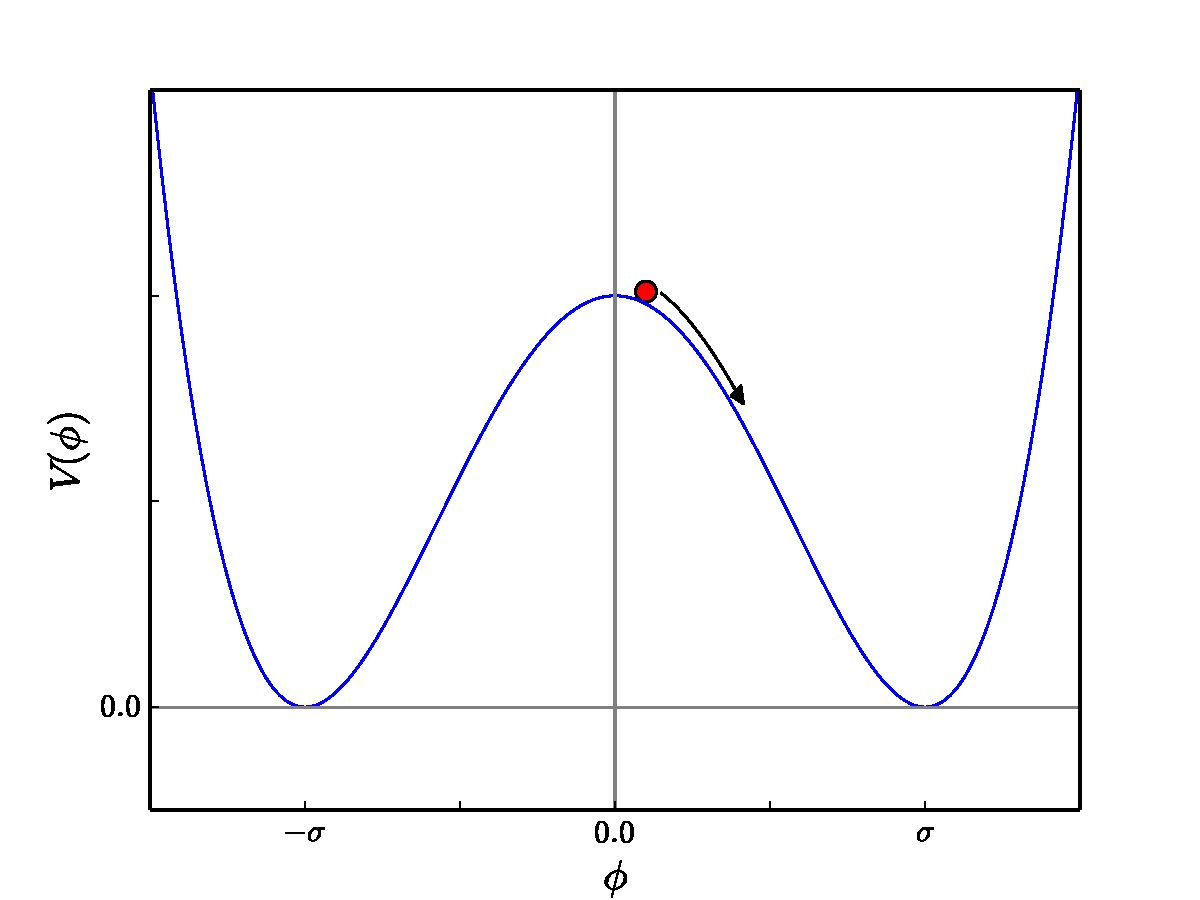
\includegraphics[width=0.75\textwidth]{figures/hilltop_cartoon.pdf}
	\caption[Schematic illustration of a Hilltop Model]{A schematic illustration of a hilltop potential, using the example of a Mexican Hat potential: $V(\phi)=\lambda(\phi^2-\sigma^2)^2$. The red ball symbolizes the inflationary field at a given time. The field rolls down the hill of the potential and settles in the vacuum state where the potential is zero, causing inflation to end. Note that in this scenario, the most inflation occurs at small values of $\phi$ and hence any hilltop model can be reasonably approximated by the first few lowest order terms.}
	\label{fig:MexHatCartoon}
\end{figure}

As an example, consider the potential in Figure \ref{fig:MexHatCartoon}, which shows a potential colloquially called the ``Mexican hat'' potential: $V(\phi)=\lambda(\phi^2-\sigma^2)^2$. For this potential, the extremum at $\phi=0$ is referred to as the false vacuum. At this value of the field, the universe is inflating. However, since the false vacuum is unstable, the field will ``roll down the hill'' of the potential and end up at the true vacuum, $\phi=\sigma$. When the inflationary field settles in the true vacuum (which is stable), the inflationary period ends. Potentials like this which have a false vacuum at $\phi=0$ are called hilltop models. For hilltop models, the inflationary period is dominated by inflation at small values of $\phi$. Hence, in a polynomial expansion of the field the lowest order terms will dominate. Thus, the potential will have only a handful of parameters (corresponding to the coefficients of the lowest order terms) requiring constraint. However, as will be discussed in Section \ref{sec:Planck}, such models do not reproduce observational results.

\begin{figure}[h]
	\centering
	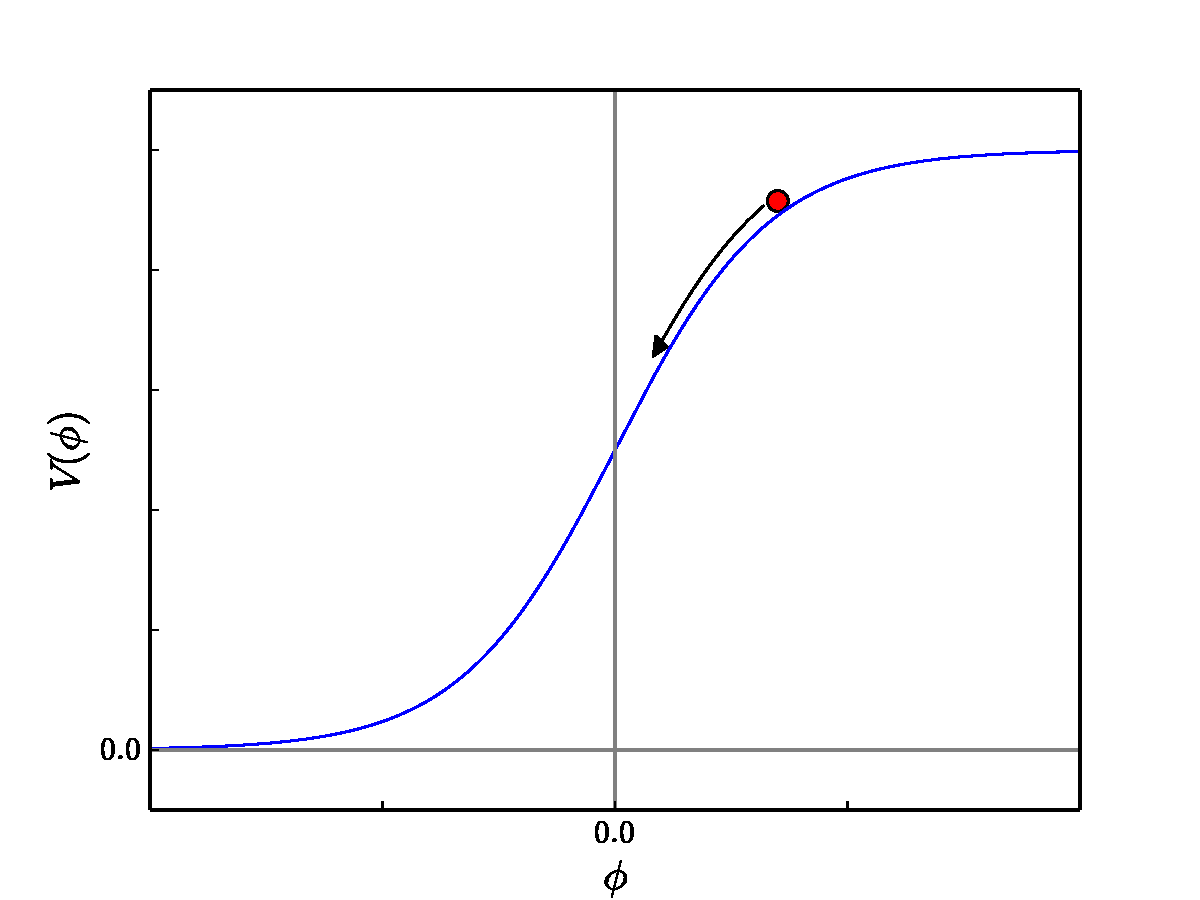
\includegraphics[width=0.75\textwidth]{figures/plateau_cartoon.pdf}
	\caption[Schematic illustration of a Plateau Model]{A schematic illustration of a plateau potential. The red ball symbolizes the inflationary field at a given time. The field rolls down the hill of the potential and settles in the vacuum state where the potential is zero, causing inflation to end. Note that in this scenario, the most inflation occurs at large values of $\phi$. Therefore, unlike in the hilltop case, the highest order terms will dominate.}
	\label{fig:PlateauCartoon}
\end{figure}

Another type of inflationary potential, which happens to be the form most in line with current observations, is the plateau model, shown in Figure \ref{fig:PlateauCartoon}. In this inflationary scenario the field begins at a large value of $\phi$ where the potential is nearly flat. The field then rolls down the hill towards smaller values of $\phi$, with inflation ending when the potential levels off to zero. Plateau models are examples of large-field models, in which the inflationary period is dominated by inflation at large values of $\phi$. Unlike in the hilltop case, inflation in the large-field models depends heavily on the higher order terms of the potential's expansion. Since small perturbations in the higher order terms will result in drastically different behavior, the potential requires an infinite number of constraining parameters. We will explore the sensitivity of such models to higher-order perturbation in Section \ref{sec:LFP}, arguing that this sensitivity reveals an undesirable amount of fine-tuning in such models of inflation.

The main purpose of an inflationary theory is to provide a mechanism to explain the homogeneity, isotropy, and flatness of the universe. As such, it is useful to look at the production of density perturbations during the inflationary period. During inflation, the magnitude of the density perturbations are inversely proportional to $\dot \phi$. Consequently, in regions where the potential is approximately constant, the perturbations would be unacceptably large. However, steeply-sloped potentials would cause the field to roll off the hill and end inflation before enough expansion took place. Therefore, there is a balancing game to be played in picking potentials. 

As we will see in the sections to come, this game of picking potentials to predict observations stumbles across many obstacles. Since the introduction of inflationary theory 34 years ago, many inflationary potentials have been proposed. However, once they satisfy observations, we have no natural criteria for choosing which among them is the ``true'' potential describing the inflationary field. 

In this paper we explore in the manner of \citet{Boyle+2006} a method of quantifying the amount of fine-tuning in an inflationary potential by counting the number of zeros in the equation of state and its derivatives. We find that \hl{...} We also explore a new method of quantifying the amount of fine-tuning in large field models that takes into account the sensitivity of the model to perturbations in higher-order terms. We find that \hl{...}

\subsection{History of Inflationary Theory}
\label{sec:History}
Inflationary theory was first proposed by Alan Guth as a possible solution to the horizon and flatness problems \citep{Guth1981}. At the time, the standard cosmological model of the early universe was an adiabatically expanding, radiation-dominated universe. This model had two fundamental problems: the horizon problem and the flatness problem, discussed in more detail in Sections \ref{sec:horizon} and \ref{sec:Flatness}. Guth's inflationary model, which proposed a period of exponential expansion in a false vacuum due to supercooling during cosmological phase transitions, solved both the horizon and flatness problems.  However, later work by Guth and Weinberg \citep{Guth+Weinberg1983} showed that the transition could not be smoothly completed in such a way that would result in a space homogeneously filled with the new phase. Further, a random region within the inhomogeneous space would be unlikely to resemble our own universe. 

Andre Linde addressed these problems with a new inflationary theory in which inflation doesn't occur at the false vacuum but rather as the inflationary field rolled down the hill of the potential towards the true vacuum. \mep{Find Citation to presentation in 1981} A similar theory was simultaneously developed by \citet{Albrecht+Steinhardt1982}. This new inflation resolved the problem of the inhomogeneities because, as mentioned in Section \ref{sec:GeneralDescription}, density fluctuations are inversely proportional to $\dot \phi$. Guth's previous model resulted in deSitter expansion, which corresponds to $\phi=const$, and hence results in unphysically large density fluctuations. Since in this new model inflation occurs as the field rolls down the hill, $\dot \phi \neq 0$ and perturbations can be made small enough to be physical. 

Although the new inflationary model solved some of the problems with Guth's original proposal, new inflation still came with issues of its own. For instance, the inflation field in the new theory often could not begin in thermal equilibrium with other fields, invalidating the use of cosmological phase transitions, which formed the basis of new inflation theory \citep{Linde2000}. Also, in the new inflationary scenario, inflation can only begin after at a time at least six orders of magnitude later than the Planck time, which is the order of a typical lifetime for a hot, closed universe \citep{LindeBook2005}. These problems, together with others, suggested that new inflation needed to be replaced with an even newer theory. 

\citet{Linde1983} proposed such a theory, called chaotic inflation, which forms the basis for most modern theories of inflation. Chaotic inflation solves the problems of its predecessors by initiating inflation for any\hl{?} initial conditions -- even conditions without thermal equilibrium or at the Planck density \citep{LindeBook2005}. In chaotic inflation, the inflaton field begins at a point far from the minimum of the potential. The field equation for chaotic inflation includes a viscosity term $\propto H \dot \phi$, so when the universe is expanding rapidly, the inflaton field rolls slowly down the potential, with the energy density of the field approximately constant. This ``slow roll'' inflation causes the universe to expand $\propto e^{Ht}$. This exponential inflation solves most problems of previous theories because all inhomogeneities in the original universe get stretched $\sim 10^{10^{12}}$ times after only $10^{-35}$s of inflation. (For comparison, the radius of the observable universe is on the order of $10^{28}$cm.) Additionally, this solves the flatness problem because even if the universe originally had a small radius of curvature, after inflation that radius is effectively infinite compared to the radius of the observable universe. \citep{Linde2000} 
%Although several more theories of inflation have been proposed (e.g. hybrid inflation, which combines two scalar fields of chaotic inflation), most are heavily based on the theory of chaotic inflation.

However, chaotic inflation still retains a particularly insidious problem, that of eternal inflation and an inflationary multiverse. Upon closer examination, it has been found that models with large scalar fields during the inflationary period produce large quantum fluctuations in the field. These fluctuations cause the local rate of inflation to change, possibly increasing the rate of inflation (equivalently, delaying the end of inflation) in a certain region. As that region expands, quantum fluctuations in that region can also cause another local section to inflate faster, and this process continues ad infinitum. Thus, once inflation begins, quantum fluctuations preclude it from ending in all regions of space. Further, due to the overwhelming expansion that occurs during inflation, the volume of space that remains inflating completely dominates the volume in which inflation ends.

To make this a little more precise, consider a region of space of radius $r$ that is undergoing exponential expansion: $a(t) \propto e^{Ht}$. The furthest distance a point in that region could influence is $H^{-1}$, so if $r>H^{-1}$, then that region can be considered its own universe.\footnote{The event horizon is defined as $d_e(t) = a(t) \int^{\infty}_t \frac{\d t}{a}$.} Following the calculation in \citet{Linde+1994}, we find how much the volume of a region of radius $H^{-1}$ increases during a time interval $H^{-1}$. During that time, the field will decrease due to its classical motion by $\Delta \phi = \tfrac{1}{4\pi \phi}$. However, the average amplitude of quantum fluctuations in the field are $|\delta \phi| = \tfrac{H}{2\pi}$. Therefore, for large enough values of $\phi$, the quantum fluctuations will dominate over the classical decrease in the field. In fact, further calculation shows that in the time $H^{-1}$, the region grows into $e^3\sim20$ disconnected domains and that in half of those domains the inflationary field will grow. Thus, the growth of the number of disconnected domains with increasing $\phi$ grows as $\propto e^{(3-\ln2)Ht}$. Also, it turns out that, regardless of the initial value of 

\subsection{Horizon Problem}
\label{sec:horizon}
Simply put, the horizon problem is the realization that the universe is homogenous and isotropic on scales far larger than the particle horizon (the farthest distance from which a point could ever receive information, given the age and expansion rate of the universe). The particle horizon is defined as 
\begin{equation}
d_p(t) = a(t) \int_0^t \frac{\d t}{a(t)},
\label{eqn:particle_horizon}
\end{equation}
where $a(t)$ is the scale factor of the universe, normalized to 1 at the present time. Consider a radiation-dominated universe, which is governed by the Friedmann equation:
\begin{equation}
H^2 = \left ( \frac{\dot a(t)}{a(t)} \right ) ^2 = \frac{8 \pi G}{3} \frac{\rho^0_r}{a^4}.
\end{equation}
Integrating this equation finds $a(t) \propto t^{1/2}$. Putting this into equation (\ref{eqn:particle_horizon}) finds that $d_p(t) = 2t \propto a^2$. Now, the size of any homogenous region is proportional to $a$. Therefore, at very small times (e.g. the Planck time), the size of the particle horizon will necessarily be smaller than the size of any homogenous region. This is a problem because, in order for a homogenous region to make sense, there must be a time at which the size of the homogenous region was smaller than the particle horizon. 

Observations of the CMB show the universe to homogenous to [Insert ridiculously small scale here], giving the homogenous region a size $l \sim c t_*$, where $t_*$ is the age of the universe at decoupling. The size of the homogenous region it must have originated from must have a size greater than $l_i \sim c t_* \tfrac{a_i}{a_*}$. However, the size of the particle horizon at that time was $l_h \sim c*t_*$. Therefore, comparing the two sizes, we find
\begin{equation}
\frac{l_i}{l_h} \sim \frac{a_i}{a_*} \sim \frac{T_*}{T_i}.
\end{equation}
 Taking $T_i$ to be the Planck temperature ($\sim 10^{32}$K) and $T_* \sim $

\subsection{Flatness Problem}
\label{sec:Flatness}

%%%%%%%%%%%%%%%%%%%
%		Math Descript	
%%%%%%%%%%%%%%%%%%%
\newpage
\section{Mathematical Description of Inflationary Theory}
\subsection{Inflationary Friedmann equation}
\label{sec:InflationaryFriedmann}
To see how one could implement an inflationary theory, let us first examine a non-inflationary Friedmann equation:
\begin{equation}
H^2 = \left ( \frac{\dot a(t)}{a(t)} \right ) ^2 = \frac{8 \pi G}{3} \left [ \frac{\rho^0_m}{a^3} + \frac{\rho^0_r}{a^4} + \Lambda + \frac{\sigma^2}{a^6} + \frac{K}{a^2} \right ]
\end{equation}
where $\rho^0_m$ is the energy density of matter in the universe at time $t=0$ (set to be the present time), $\rho^0_r$ is the current energy of radiation, $\Lambda$ is the cosmological constant, $\sigma$ is the cosmic anisotropy term, and $K$ is the curvature of the universe. As we can see by examining the powers of $a$ in each term, the early universe is dominated by the anisotropy term, $\propto a^{-6}$, while the late universe is dominated by the curvature term (and cosmological constant). Therefore, the simplest way to add inflation to the model of the universe is to add an inflationary term to the Friedmann equation: 
\begin{equation}
H^2 = \left ( \frac{\dot a(t)}{a(t)} \right ) ^2 = \frac{8 \pi G}{3} \left [ \frac{\rho^0_m}{a^3} + \frac{\rho^0_r}{a^4} + \Lambda + \frac{\sigma^2}{a^6} + \frac{K}{a^2} + \frac{\rho^0_\phi}{a^{2\epsilon}} \right ]
\end{equation}
where $\rho^0_\phi$ is the energy density of the inflationary field and $\epsilon$ is a positive exponent. In order to ensure that the universe expands during the inflationary period, we must constrain the value of $\epsilon$. 
%that must satisfy $\epsilon<1$ for inflation to dominate in the early universe. (Note: $\epsilon>3$ would cause contraction in the early universe.) 
%\mep{I have in my notes that $\epsilon<1$ for inflation and $\epsilon>3$ for contraction, but that doesn't make sense, so I think that's wrong.} 
%Now using this form for the inflationary term, 
To do so, we must examine how an inflation-dominated universe would evolve. In a $\phi$-dominated universe, the Friedmann equation becomes:
\begin{equation}
H^2 = \left ( \frac{\dot a}{a} \right ) ^2 = \frac{H_0 \Omega_\phi}{a^{2\epsilon}},
\label{eqn:Friedmann_phi}
\end{equation}
where $H_0$ is the Hubble constant and $\Omega_\phi = \tfrac{8\pi G \rho_\phi}{3 H_0}$. Now, solving this equation for $a(t)$ gives
\begin{equation}
a(t) \propto (\epsilon \sqrt{H_0 \Omega_\phi} t)^{1/\epsilon},
\label{eqn:inflation_a(t)}
\end{equation}
and hence 
\begin{equation}
\ddot a(t) \propto \left ( \frac{1-\epsilon}{\epsilon} \right ) (H_0 \Omega_\phi)^{1/2\epsilon} t^{\tfrac{1-2\epsilon}{\epsilon}}. 
\end{equation}
From this, we can see that the condition for an expanding universe is $\epsilon<1$. 
%\mep{Shoot. So my notes must have been right. But how can a small power in the denominator dominate at small values of a? That doesn't make sense!?!? Also, I know for a fact that the radiation term dominates before matter. So to be consistent with that, higher (negative) powers dominate earlier.} 
However, note that at arbitrarily early times (small values of $a$), the anisotropy term will dominate. Thus, in order for inflation to dominate during early times, the value of $\rho^0_\phi$ compared to $\sigma^2$ and the other coefficients must be specified such that at the Planck scale the inflationary term will dominate. %Therefore, we want to find an inflationary theory that produces an inflationary term in the Friedmann equation $\propto a^{-2\epsilon}$ so that the universe will be dominated by expansion at early times. 
Also, it is important to note that, in order for inflation to end, $\epsilon$ must grow to become greater than one, so we know that $\epsilon$ should be time-dependent. 

\subsection{Inflationary Field \& Equation of State}

In order to derive a field theory that will produce such an inflationary term consistent with the requirements detailed in Section \ref{sec:InflationaryFriedmann}, we turn to the equation of state, $w=\rho/p$, where $\rho$ is the energy density and $p$ is the pressure of the field. The equation of state is related to $\epsilon$ by the equation 
\begin{equation}
\epsilon = \tfrac{3}{2}(w+1). 
\label{eqn:eps_w}
\end{equation}
Thus, an inflationary field must have an equation of state $w<-1/3$. Table \ref{tab:field_scenarios} summarizes the values $w$ and $\epsilon$ and the evolution of $a(t)$ for different types of fields. 

\begin{table}[htbp]
   \centering
   \begin{tabular}{@{} lcccc @{}} % Column formatting, @{} suppresses leading/trailing space
      \toprule
      Field Type & $w=\rho/p$ &  $\epsilon=\tfrac{3}{2}(w+1)$ & $a(t)$ & $\ddot a(t)$ \\
      \midrule
      matter & 0 & $3/2$ & $\propto t^{2/3}$ & $>0$ \\
       radiation & $1/3$ & $2$ & $\propto t^{1/2}$ & $<0$ \\
       $\Lambda$ & $-1$ & $0$ & $\propto e^t$ & $>0$ \\
       inflation & $<-1/3$ & $<1$ & $\propto t^{1/\epsilon}$ & $>0$ \\
       contraction & $>1$ & $>3$ & $\propto t^{1/\epsilon}$ & $<0$ \\
      \bottomrule
   \end{tabular}
   \caption{The values of $w$ and $\epsilon$ and the evolution of $a(t)$ for different types of fields.}
   \label{tab:field_scenarios}
\end{table}


From Table \ref{tab:field_scenarios}, we see that an inflationary field must have an equation of state $w<-1/3$. From this, we want to put constrains on the Lagrangian density $\L$ for the inflationary field. Let $\phi$ be an inflationary field. Its Lagrangian density takes the form:
\begin{equation}
\L = -\half ( \partial_\mu \phi)^2 - V(\phi)
\end{equation}
Using the assumptions that $\phi$ is homogenous (so that $\partial_j \phi = 0$) and isotropic (so that we can use the Minkowski metric $\eta_{\mu\nu}$), we find that the stress-energy tensor of the field is
\begin{equation}
T_{\mu\nu} = -\eta_{\mu 0} \dot \phi^2 + \eta_{\mu\nu}(\half\dot \phi^2+V(\phi)).
\end{equation}
From this, we find that the equation of state is
\begin{equation}
w = \frac{\half \dot \phi^2 - V(\phi)}{\half \dot \phi^2 + V(\phi)}.
\label{eqn:w}
\end{equation}
Putting in the constraint on $w$ for inflation, we find that an inflationary field must satisfy 
\begin{equation}
\dot \phi^2 < V(\phi).
\end{equation}
\mep{Is this important? It seems it should be, but we never talked about it before...}

Once we have $\L$, we know that the equation of motion for the field is the Klein-Gordon equation:
\begin{equation}
\ddot \phi + 3H \dot \phi + V'(\phi) = 0,
\label{eqn:KG}
\end{equation}
where $H$ is the Hubble parameter, $V(\phi)$ is the inflationary potential, and a dot indicates a time derivative. In our convention, the reduced Planck mass is set to one, i.e. $M_{pl} = (8\pi G)^{-1/2} \equiv 1$. Combining this with the Friedmann equation, 
\begin{equation}
H = \sqrt{\tfrac{1}{3} \left ( \half \dot \phi^2 + V(\phi) \right )},
\label{eqn:Friedmann}
\end{equation}
completely determines the evolution of a universe dominated by an inflationary potential $V(\phi)$. It will be useful later on to re-write the Friedmann equation in terms of $\epsilon$. Putting together equations (\ref{eqn:Friedmann_phi}) and (\ref{eqn:inflation_a(t)}), we find that
\begin{equation}
\epsilon = -\frac{\dot H}{H}
\label{eqn:Friedmann_epsilon}
\end{equation}
Note that, for general inflationary potentials, $\epsilon$ will not be constant in time. This is fortuitous since, in order for inflation to end, $\epsilon$ will have to go from a value greater than 1 to a value less than 1. We can also use this equation to further constrain the inflationary potential with a ``graceful exit'' condition. \mep{I think this is true. I need to look up more info \& elaborate.}

\subsection{Calculating Observable Parameters}
Of course, the whole point of creating an inflationary theory is to be able to reproduce observational data. When observations from experiments such as WMAP and Planck observe the early universe, they measure the power spectrum of density fluctuations in the primordial plasma. \mep{More elaboration on where these come from}

Instead of working in units of time, where the time at the end of inflation is difficult to pinpoint, we choose instead to work in terms of the number of e-folds until the end of inflation, defined as 
\begin{equation}
N = -\int_t^{t_{end}} H \d t \text{\ \ \ or\ equivalently\ \ \ } \d N = -H \d t. 
\label{eqn:defN}
\end{equation}
Note that $N$ runs backwards in time, so as time increases the number of e-folds decreases. In these units, the end of inflation is defined to occur at $N=0$, so at this time $\epsilon=1$. Current observations look at a narrow window centered on $N=60\equiv N_*$.  

Figure \ref{fig:density_fluctuations} shows a schematic of the density fluctuations as a function of the wavenumber of the fluctuations ($\log k\sim\tfrac{1}{N}$). If the fluctuations were purely scale invariant, then the curve would be a horizontal line, the amplitude of the fluctuations independent of their wave number. Since current observations see only a very limited range near $N_*$, so they focus on measuring (and we focus on predicting) the deviation from scale invariance at that point. This deviation is called the spectral tilt, denoted $n_s(k^*)$, where $k^*$ is the value of $k$ at $N_*$. Following the work of \citet{Wang+1997}, we use an approximation of the spectral index to first order in $\epsilon$:
\begin{equation}
n_s \approx 1 - 2\epsilon - \frac{\d \ln(\epsilon)}{\d N} + \mathcal{O}(\epsilon^2),
\label{eqn:ns_def}
\end{equation}
where the equation of state is treated as a function of the number of e-foldings instead of a function of time. 

In addition to the spectral tilt at $N_*$, observations can also constrain the tensor-to-scalar power ratio, typically denoted $r$. The tensor-to-scalar ratio is typically computed in the slow-roll approximation (See Section \ref{sec:SlowRoll} for more details), and we follow the conventions of \citet{Planck2013} to get 
\begin{equation}
r \approx 16 \epsilon.
\end{equation}


\subsection{Fine-tuning in an Inflationary Theory}
Now that we have the basic mechanics of an inflationary theory, we see that defining an instance of an inflationary theory reduces to defining the inflationary potential $V(\phi)$. In order for inflation to be a predictive theory, we need to find a way to choose which potentials are reasonable and then find whether any of those potentials would generate a universe that conforms with observations. 


\subsection{Slow Roll Approximation}
\label{sec:SlowRoll}
In the slow roll approximation, we assume that $\dot \phi$ and $\ddot \phi$ are small. In order for this to be true, the inflationary potential must not be varying rapidly, leading us to the slow roll approximations:
\begin{equation}
\left | \frac{V'(\phi)}{V(\phi)} \right | <<1 \text{\ \ \ and\ \ \ } \left | \frac{V''(\phi)}{V(\phi)} \right | <<1 .
\label{eqn:SlowRollApprox}
\end{equation}
With these approximations, the Friedmann equation becomes
\begin{equation}
3 H^2 \approx_{sr} V(\phi),
\label{eqn:Friedmann_sr}
\end{equation}
and the Klein-Gordon equation becomes
\begin{equation}
3 H \dot \phi \approx_{sr} -V'(\phi)
\label{eqn:KG_sr}
\end{equation}
We use these approximations to find the initial conditions for integrating equation (\ref{eqn:KG_N}): $\phi(N=0)$ and $\dot \phi(N=0)$. To do this, we use the fact that, at the end of inflation (i.e. at $N=0$), $\epsilon = 1$. Recall from Section \ref{ssec:InflationaryFriedmann} that the condition for accelerated expansion is $\epsilon<1$. Therefore, as the universe transitions out of the inflationary epoch and into a period of decelerating expansion (where $\epsilon>1$), there must be a point where $\epsilon=1$, marking the end of inflation. Putting together equations (\ref{eqn:eps_w}) and (\ref{eqn:w}), we find that 
\begin{equation}
\epsilon = \frac{3}{2} \left ( \frac{\dot \phi^2}{\half \dot \phi^2 + V(\phi)} \right ) \approx_{sr} \half \left (\frac{V'(\phi)}{V(\phi)} \right ) ^2 
\label{eqn:eps_sr}
\end{equation}
where we have used the slow roll approximations $\half \dot \phi^2 << V(\phi)$ and equation (\ref{eqn:KG_sr}). Setting $\epsilon=1$ gives us an equation we can solve for $\phi(N=0)$. Once we have $\phi(N=0)$, we can easily us equation (\ref{eqn:KG_sr}) to find $\dot \phi(N=0)$. 

%%%%%%%%%%%%%%%%%%%
%		Methodology	
%%%%%%%%%%%%%%%%%%%
\newpage
\section{Methodology}
\label{sec:methods}
\subsection{Description of Code Equations}
Let $\phi$ be an inflationary field governed by equations (\ref{eqn:Friedmann}) and (\ref{eqn:KG}). For the purposes of our code, we find it easier to work with $\phi$ not as a function of time but rather as a function of the number of e-folds until the end of inflation, defined in equation (\ref{eqn:defN}). If we let $\dot \phi$ denote the derivative of $\phi$ with respect to $t$ and $\phi'$ denote the derivative of $\phi$ with respect to $N$, then we have $\dot \phi = -H \phi'$. Using this relation, the Friedmann equation becomes
\begin{equation}
H^2 = \frac{V(\phi)}{3 - \half(\phi')^2},
\end{equation}
and the Klein-Gordon equation becomes 
\begin{equation}
2H^2\phi'' + H^2(\phi')^3 - 6H^2\phi' + 2V'(\phi) = 0.
\label{eqn:KG_N}
\end{equation}
Conveniently, when we use this formulation, the equation of state reduces from its exact form to
\begin{equation}
\epsilon = \frac{3 \dot \phi^2}{\dot \phi^2 + 2 V} = \phi'^{2},
\label{eqn:eps_N}
\end{equation}
and the spectral tilt from Eq. \ref{eqn:ns_def} becomes
\begin{equation}
n_s = 1 - \phi'^2 + 2\frac{\phi''}{\phi'}.
\label{eqn:ns_N}
\end{equation}
Therefore, in order to find the observational predictions of different inflationary models, we just need to solve Eq. \ref{eqn:KG_N} for $\phi(N)$, plug that into Eqs. \ref{eqn:eps_N} and \ref{eqn:ns_N}, and then find $n_s$ and $r$ at $N=60$. Since Eq. \ref{eqn:KG_N} is not usually analytically solvable for a give potential $V(\phi)$, we used Mathematica to numerically solve the system. 

\subsection{Discussion of Initial Conditions and Convergence}

This leads us to the problem of initial conditions. In order to solve this second-order differential equation, we need two bounds, which we chose to be $\phi(N=0)$ and $\phi'(N=0)$. We can get approximate values by using the slow-roll approximation, setting $\epsilon=1$ and solving Eq. \ref{eqn:eps_sr} for $\phi(N=0)\equiv \phi_{i,1}$. Next we combine Eqs. \ref{eqn:eps_sr} and \ref{eqn:eps_N} to find that 
\begin{equation}
\phi' = \pm \frac{V'(\phi)}{\sqrt{2}V(\phi)},
\end{equation}
where the prime on $\phi$ denotes a derivative with respect to $N$ but the prime on $V$ denotes a derivative with respect to $\phi$. This allows us to find $\phi'(N=0)\equiv \phi p_{i,1}$. Using $\phi_{i,1}$ and $\phi p_{i,1}$ as initial conditions, we numerically integrate up the slope of the potential back to $N_f=80$ efoldings. (Although our purpose is to find $n_s$ and $r$ at $N_*=60$, integrating back to $N_f=80$ gives us a numerical cushion.) 

However, using the slow-roll approximation for the initial conditions is not ultimately accurate enough for our purposes. To check the validity of our solution $\phi_{s,1}(N)$, we put this solution into the exact expression for $\epsilon(\phi)$ (Eq. \ref{eqn:eps_N}) and find $\epsilon(N=0)$. If our solution were exactly accurate, we would expect $\epsilon(N=0)=1$. However, we find that this first solution for $\phi(N)$ is typically off by a few efoldings, with $\epsilon=1$ occurring at a value of $N$ typically between $-1$ and $-3$. Therefore, in order to force $\epsilon(N=0)$ to be one, we shift our solution $\phi_{s,1}(N)$ by $N_1$ where $\epsilon(\phi_{s,1}(N_1))=0$. Then we use $\phi_{i,2} = \phi_{s,1}(N_f+N_1)$ and $\phi p_{i,2} = \phi_{s,1}'(N_f+N_1)$ for our new initial conditions, resulting in a new solution $\phi_{s,2}(N)$. In order to check the convergence of our method, we find another solution by using the values of $\phi_{s,2}(N_f)$ and $\phi_{s,2}'(N_f)$ as new initial conditions to numerically solve the differential equations yet again. We then check that the two solutions are the same (up to numerical precision). If they are not the same, we repeat the procedure until there is convergence upon a solution $\phi_s(N)$.

To summarize our numerical method, first we use the slow roll to approximate $\phi$ and $\phi'$ at $N=0$.  Next we integrate back up the hill of the potential to find the solution between $N=0$ and $N_f$. Then we shift the solution so that $\epsilon$ is one at $N=0$ and integrate back down the hill from $N_f$ to $N=0$. If necessary, we repeat this process until convergence. Once we have the final, converged solution $\phi_s(N)$, we can compute the observables $n_s$ and $r$ using Eqs. \ref{eqn:ns_N} and \ref{eqn:eps_N}, respectively.



%%%%%%%%%%%%%%%%%%%
%			Planck	
%%%%%%%%%%%%%%%%%%%
\newpage
\section{Current Status of Models and Observation}
\label{sec:Planck}

\subsection{Current Observations}
To date, a myriad of potentials have been proposed as possible models of inflation. We use the numerical methods described in Section \ref{sec:methods} to find the observational predictions of the most prominent classes of proposed models and we compare these theoretical results to the observational results of \citet{Planck2015}. 

Figure \ref{fig:Planck} shows a plot on the \nsr plane of the theoretical predictions of many different proposed models of inflation. These are overlaid on approximate Planck data contours from the \citet{Planck2015} results. The contours mark the $68\%$ and $95\%$ confidence regions for the combined TT, TE, EE, and lowP results. For each inflationary model we find the predictions for $n_s$ and $r$ at $N=60$ (the large markers) and at $N=50$ (the small markers). The sweeping regions of color are used for models that have a free parameter and cover the region spanned by varying the free parameter. At each value of the parameter, a bar is drawn between the $N=50$ and $N=60$ points in the \nsr plane. The following sections (\ref{ssec:SmallField} and \ref{ssec:LargeField}) contain more detailed analysis of each class of inflationary potential in Figure \ref{fig:Planck}. 

\begin{figure}[h]
	\centering
	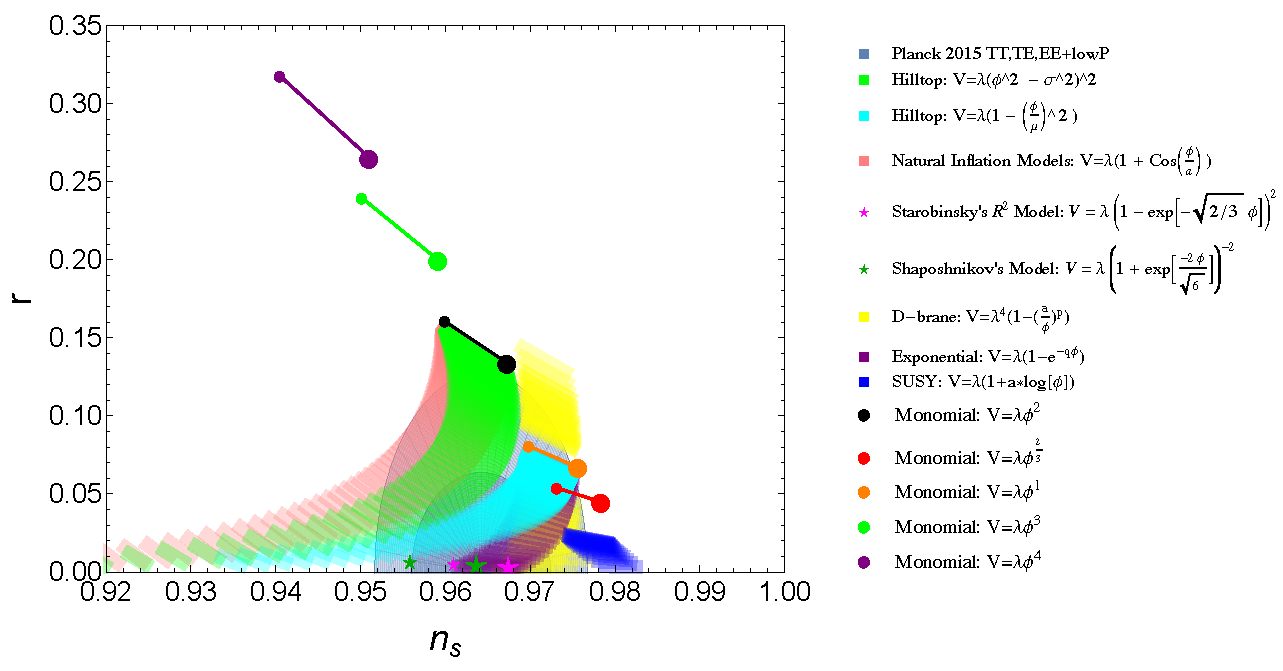
\includegraphics[width=\textwidth]{figures/PlanckPlotLegendsFinal.pdf}
	\caption[Coverage in the \nsr plane of proposed models of inflation.]{A plot of the coverage in the \nsr plane of different proposed models of inflation. For the monomial plots, the large point markers represent the values at $N=60$, and the small point markers represent the values at $N=50$. For models with a free parameter, such as Hilltop, Natural Inflation, Exponential, and SUSY, the shaded regions show the area covered by varying the free parameter for $N$ between 50 and 60. Underneath the model regions are approximate contours showing the constraints placed on $n_s$ and $r$ by the \citet{Planck2015} results.}
	\label{fig:Planck}
\end{figure}

\subsection{Small Field Models}
\label{ssec:SmallField}

\subsubsection{Polynomial Hilltop Models}
\label{sssec:Hilltop}
Perhaps the simplest class of small field inflationary models is the set of polynomial hilltop potentials. We examined two different forms for these potentials, a ``Mexican Hat'' form, 
\begin{equation}
V(\phi)=\lambda(\phi^2-\sigma^2)^2,
\end{equation} 
and a quadratic form, 
\begin{equation}
V(\phi)=\lambda(1-(\tfrac{\phi}{\mu})^2)
\end{equation} 
\citep{Boubekeur+Lyth2005}. Both of these models belong to the class of small field inflationary models, in which inflation begins at small values of $\phi$ and rolls down the hill to a vacuum at a larger value of $\phi$. Whenever doing calculations with these models, we first shift the potential so that the false vacuum (the minimum of the potential) falls at $V=0$. As discussed previously, this ensures that inflation ends. 

For large values of $\sigma$, the $n_s$ and $r$ values for the Mexican hat potential converge on the values for the monomial $\phi^2$ potential. This is expected since large values of $\sigma$ will cause the $-2\sigma^2\phi^2$ term to dominate over the $\phi^4$ term, and shifting the potential minimum to $V=0$ will offset the increase in the $\sigma^4$ term. For large value of $\mu$, the $n_s$ and $r$ values for the quadratic form converge on the linear $V\propto \phi$ model. 

\subsubsection{Natural Inflation Model}
Natural inflation is another form of a hilltop model and takes the form:
\begin{equation}
V(\phi)=\lambda(1+\cos(\tfrac{\phi}{a}))
\end{equation}
\citep{Adams+1993}. It is theoretically motivated as a mechanism for inflation in which the inflationary period ends for $\phi\gg M_{pl}$, which is $1$ in our units. In the particle theory behind natural inflation, $\phi$ is a pseudo-Nambu-Goldstone boson with a periodic potential and a scale of spontaneous symmetry breaking that is much greater than $M_{pl}$ \citep{Boubekeur+Lyth2005}. For large values of $a$, the results for natural inflation converge on the results for a second degree monomial, $V\propto\phi^2$, similar to the case of the Mexican hat potential. Again, this is expected due to the series expansion of the cosine. 

\subsection{Large Field Models}
\label{ssec:LargeField}

\subsubsection{Monomial Models}
\label{sssec:Mono}
The simplest large field models of inflationary potentials are monomial power laws: 
\begin{equation}
V(\phi)=\lambda\phi^n,
\end{equation} 
for some positive $n$. These models, specifically the $\phi^4$ model, were first explored by \citet{Linde1983} as an example of chaotic inflation. Monomial models are large-field models (meaning that the inflationary field begins at large values of $\phi$ and rolls down the hill to a vacuum at a smaller value of $\phi$. For the monomial models, the vacuum state is at $\phi=0$. Note that for potentials where $n$ is not an even integer there is no minimum value of the potential and hence no vacuum state. Potentials that are not bounded below are problematic because inflation ends when the inflationary field settles in the vacuum state. Without a stable vacuum state, the inflationary field will enter a negative regime of the potential, and the universe will collapse. However, it is still instructive to examine these unbounded models since they can still serve as upper limits on other classes of models, such as $V=\lambda\phi$ for the Hilltop models (see Section \ref{sssec:Hilltop}).

\subsubsection{Exponential Model}
Exponential inflation was first proposed by \citet{Goncharov+Linde1984} as a chaotic inflation model derived from the framework of $N=1$ supergravity, and has recurred many times in inflationary models grounded in other theories of supergravity and string theory. Its potential takes the form
\begin{equation}
V(\phi)=\lambda(1-e^{-q\phi}).
\end{equation} 
For small values of $q$, the model converges on the results for the linear monomial, as expected from the series expansion of the exponential. Note that, as for many of the monomial potentials, the exponential potential is not bounded below. It is possible to fix this without significantly upsetting the behavior of the system during inflation by adding a small term such as $\tfrac{0.01}{x^2}$ to the potential. This gives the potential a minimum which we can then shift to occur at $V=0$. 

\subsubsection{D-brane Models}
Another breed of large field models, called D-brane models, take the form 
\begin{equation}
V(\phi)=\lambda(1-(\tfrac{a}{\phi})^p)
\end{equation} 
for some positive integer $p$, usually taken to be 2 \citep{Garcia+2002} or 4 \citep{Dvali+Tye1999}. D-brane models originate from extra-dimensional physics in which brane/anti-brane interaction drives inflation. Interestingly, we found that the power $p$ does not effect the \nsr coverage of the model. In Figure \ref{fig:Planck}, the D-brane model data used $p=1,\ 2,\ 3,\ 4$. The D-brane models do not particularly converge to any monomial, although their coverage does include the linear monomial. As in the case of the exponential potential, we must add a small term to the potential to give it a minimum and hence ensure the end of inflation.

\subsubsection{Logarithmic (SUSY) Models}
A logarithmic potential, which has a potential of the form 
\begin{equation}
V(\phi)=\lambda(1+a\log(\phi)),
\end{equation} 
can be generated by loop corrections in spontaneously broken supersymmetric (SUSY) grand unified theories \citep{Dvali+1994}. Once again, we must add a term to the potential for the end of inflation. 


\subsubsection{Starobinsky and Shaposhnikov's Models}
Two of the most promising models of inflation which fall entirely within \citet{Planck2015}'s $95\%$ constraints are Starobinsky's $R^2$ model, 
\begin{equation}
V(\phi)=\lambda\left(1-e^{-\sqrt{2/3}\phi}\right)^2,
\end{equation} 
and Shaposhnikov's model, 
\begin{equation}
V(\phi)=\lambda \left(1+e^{-\sqrt{2/3}\phi}\right)^{-2}.
\end{equation} 
Starobinsky's model is derived from one-loop corrections to conformally covariant matter fields, which then can admit nonsingular isotropic and homogeneous solutions which produce a universe in a state of de Sitter expansion \citep{Starobinsky1980}. Shaposhnikov's model is derived from introducing a non-minimal coupling of the Higgs scalar field to gravity \citep{Bezrukov+Shaposhnikov2008}. Although the series expansions of these two models are quite different (e.g. Shaposhnikov's model begins at the second order term while Starobinsky's model has zeroth and first order terms as well.), the models' results end up very close to each other on the \nsr plane.

\FloatBarrier
%%%%%%%%%%%%%%%%%%%
%			Latham	
%%%%%%%%%%%%%%%%%%%
\newpage
\section{Current Methods of Quantifying Fine Tuning}
\label{sec:Latham}

One persistent problem in inflationary theory that has generated much discussion is the problem of fine tuning. Although it is such a pervasive topic, the concept of fine-tuning is not very well defined, having multiple definitions relevant to different aspects of inflationary models. One manifestation of fine-tuning is in the smallness of constants within the inflationary model. For example, a potential of the form $V(\phi)=\tfrac{m}{2}\phi^2$ has to have $m \ll 10^{-11} M_{Pl}$ in order to conform with the observed perturbation amplitudes $\tfrac{\delta \rho}{\rho}\sim 10^{-4}$ at $\phi_{60}$.\footnote{This value was computed using $\tfrac{V''(\phi_{60})}{V(\phi_{60})}=\tfrac{1}{60}$ to solve for $\phi_{60}$ and then using $\tfrac{\delta\rho}{\rho}=\tfrac{V(\phi_{60})^{3/2}}{V'(\phi_{60})}\sim10^{-4}$ to solve for $m$ in units of the Planck mass $M_{Pl}$.} Having a mass parameter this small but still non-zero is very peculiar and thus this model is called ``fine-tuned.'' Another way to look at fine tuning is to consider the functional complexity of the evolution of physical parameters, such as the equation of state $\epsilon$. In this section we will review the work done by \citet{Boyle+2006} on quantifying such a measure of fine-tuning in polynomial potentials in preparation for proposing a new method for quantifying fine-tuning in plateau models. 

\subsection{Quantifying Fine Tuning in Polynomial Potentials}

The method for quantifying fine-tuning proposed by \citet{Boyle+2006} examines the complexity of the equation of state $\epsilon$ generated by a given potential. The motivation for using such a scheme is the realization that many inflationary potentials are only able to achieve \nsr values consistent with observations by introducing unnecessary features into the equation of state. These features are a form of fine-tuning because they introduce artificial forces and jerks right around the observational point, $N=60$. Boyle's method is as follows: 1) Solve the Klein-Gordon equation for $\phi(N)$, 2) Plug the solution $\phi(N)$ into the equation for the slow roll parameters $\epsilon$ and $\eta$, and 3) Count the zeroes in each function and its derivatives. This number, $Z_{\epsilon,\eta}$ is the degree of fine-tuning of the model. 

Figure \ref{fig:Latham} (adapted from \citet{Boyle+2006}) shows the results of the zero-counting method for polynomial potentials. Each colored swath represents the range in the \nsr plane covered by polynomial models with the degree of fine-tuning $Z_{\eta}$. The area inside the solid black curve contains all the models with degrees of fine-tuning $Z_{\eta}=0$ or 1. The small white circles denote monomial potentials: $\phi^4$, $\phi^3$, and $\phi^2$, from left to right. The hashed region contains potentials whose polynomial degree is greater than four but whose fine-tuning degree is zero. The red contour lines were added to compare \citet{Boyle+2006}'s results with the \citet{Planck2015} constraints. 

\begin{figure}[H]
	\centering
	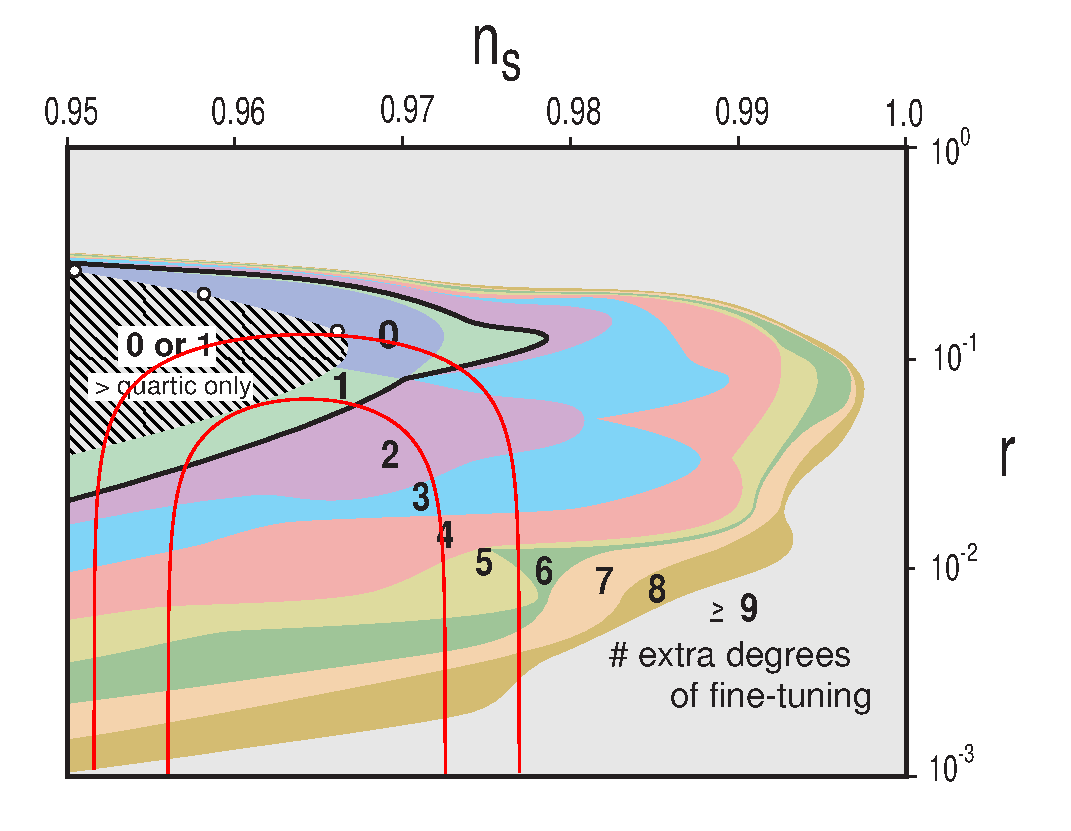
\includegraphics[width=0.7\textwidth]{figures/LathamFigurePlanck.pdf}
	\caption[Plot of \nsr coverage of polynomial models showing fine-tuning]{A plot in the \nsr plane of the observational predictions of polynomial models. The coloring tells how many zeros there are in the equation of state $\epsilon$ and its derivatives (with respect to $N$). This figure is adapted from \citet{Boyle+2006}. The red contour lines were added to depict the $68\%$ and $95\%$ confidence regions for Planck's combined TT, TE, EE, and lowP results.}
	\label{fig:Latham}
\end{figure}

Noting in Figure \ref{fig:Latham} the extent of the region within the black line, which contains the models with zero or one degree of fine-tuning, we see that the simplest models encompass only a small region of the \nsr plane. Further, there is little overlap between the \citet{Planck2015} contours and the models with the smallest degree of fine-tuning, and it is likely that as the constrains become stronger and push $r$ to lower values there will ultimately be no overlap at all. This shows that in order to get to small values of the tensor-to-scalar ratio, we must introduce fine-tuned features into the equation of state. 

    This method works well for discerning fine-tuning in the equation of state. However, the models that \citet{Boyle+2006} examines, namely polynomial models, are now generally disfavored by observations (see Section \ref{sec:Planck}). In the following section we will discuss a new method of examining the fine tuning in inflationary potentials that we apply to the large field models consistent with \citet{Planck2015} data.

%%%%%%%%%%%%%%%%%%%
%		Large Field Models	
%%%%%%%%%%%%%%%%%%%
\newpage
\section{Quantifying Fine-tuning in Large Field Potentials}
\label{sec:LFP}

While the zero-counting method works well to quantify the amount of fine-tuning in a polynomial model, we need another method to quantify the fine-tuning in the large field models, particularly the models with a plateau. For plateau models, we want to highlight the fact that in order to sustain a flat plateau out to infinity --- as most plateau models implicitly require --- we must constrain an infinite number of parameters (i.e. the coefficients of the series expansion of the model) to high precision. We do this by probing the sensitivity of the models to monomial perturbations. For each model we add a term $a\phi^p$ where $p$ is a power, typically taken to be 4 or above, and $a$ is a constant such that $a\ll 1$. We then track how the model's results move in the \nsr plane as $a$ increases. For a large enough value of $a$, the model will converge on the result for the potential $V(\phi)=\phi^p$. The amount of drift in the \nsr plane (e.g. how large $n_s$ and $r$ can become) and the value of $a$ at the maximum drift points can give us a measure for how sensitive the model is to large field perturbations. 

In the rest of this chapter, we will first explore in detail how this perturbation-drift method works in the case of the Tanh potential. Then we will compare the amount of drift from several different models to see which are more sensitive to perturbations. Finally, we will look at the effects that changing the power of the perturbing function will have on the amount of drift for a specific model. 

\subsection{Tanh Case Study}
\label{ssec:TanhCaseStudy}

In order to assess the practicality of the perturbation-drift method, we first apply the method to the plateau model $V(\phi)=1+\tanh(\phi)$. Tanh models were first proposed by \citet{Kallosh+2013} as $V(\phi)=\tanh^{2n}(\tfrac{\phi}{\sqrt{6\alpha}})$, which forms the simplest class of models with spontaneous conformal symmetry breaking. \citet{Planck2015} found that $0.02<n<1$ falls within their $95\%$ confidence levels, so we pick $n=0.5$ for convenience. The Tanh model is an appealing first choice because it is already bounded below without requiring an additional term to introduce a vacuum state. Also, since we shift the potential upwards, we rescale the potential by a constant factor so that the plateau asymptotes to $V=1$. This is done so that in later sections we can make fair comparisons between models (more discussion in Section \ref{ssec:DriftResults}). In the following discussion, all potentials are assumed to be vacuum-shifted and rescaled appropriately.

Figure \ref{fig:LFP_tanh_drift_detail} shows the drift in the \nsr plane due to quartic perturbations of the Tanh potential. The black circle shows the pure Tanh model, $V(\phi)=\tanh(\phi)$, and the cyan line traces the curve that the model follows as it is perturbed by the term $a\phi^4$ with increasing values of $a$. A perturbation of amplitude $a=3\times10^{-5}$ already takes the model outside the Planck constraint contours,  and $a=10^{-4}$ takes the model to a value of $n_s$ greater than one. This sensitivity to slight deviations from an exact Tanh model is disturbing because there are an infinite number of higher order terms in the potential that must be precisely tuned to the correct value. Otherwise the observational predictions of the model will be drastically altered. Further, as we shall see in Section \ref{ssec:DriftVaryAf}, higher order perturbing terms induce a larger effect at a smaller epsilon, heightening the problem.

\begin{figure}[H]
	\centering
	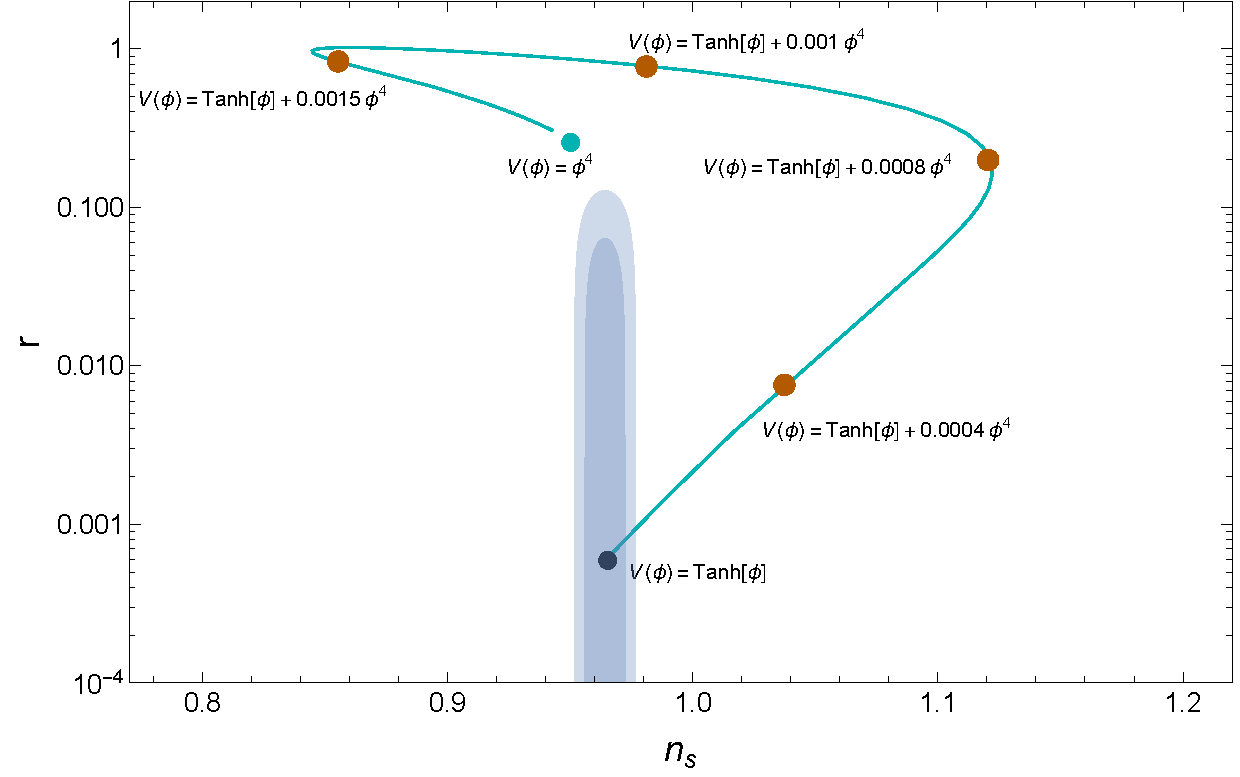
\includegraphics[width=\textwidth]{figures/TanhDriftLabeledPointsPlanck.pdf}
	\caption[Drift in \nsr plane for Tanh model with perturbations (more detailed plot).]{A plot showing the drift in the \nsr plane as a $V=\tanh(\phi)$ model is perturbed with a $\phi^4$ potential. Note that the model is shifted so that the vacuum is at $V=0$ and is rescaled by a constant factor so that the plateau asymptotes to $V=1$. The cyan circle marks the location of a pure $\phi^4$ potential, and the black circle marks the pure $\tanh(\phi)$ potential. The orange circles are labeled to show the amplitude of perturbation at different points on the curve. The light blue contours show approximate contours of the \citet{Planck2015} $68\%$ and $95\%$ constraints.}
	\label{fig:LFP_tanh_drift_detail}
\end{figure}

\begin{figure}[P]
	\centering
	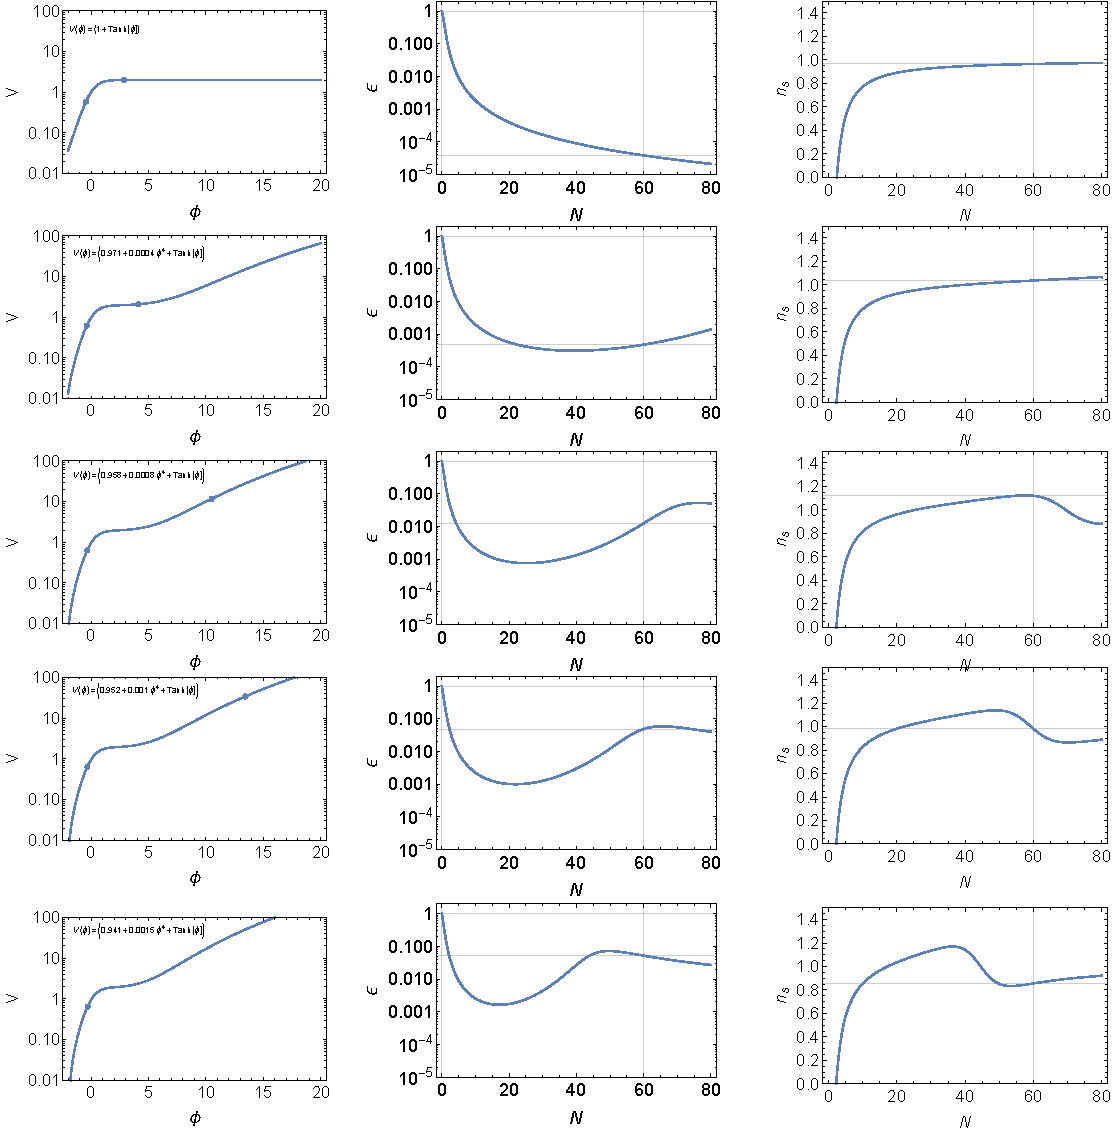
\includegraphics[width=\textwidth]{figures/Tanh_V_ns_eps_grid.pdf}
	\caption[Grid of plots showing $V$, $\epsilon$, and $n_s$ for the perturbed Tanh potentials.]{A grid of plots showing $V$, $\epsilon$, and $n_s$ for the Tanh potential with increasing amounts of perturbation. The potentials used correspond to the ones marked in Figure \ref{fig:LFP_tanh_drift_detail}. The two dots on the potential plot show the $N=0$ (left) and $N=80$ (right) marks.}
	\label{fig:LFP_tanh_grid}
\end{figure}
\FloatBarrier

These large drifts in the \nsr plane lead us to the question of what physically is happening to the potential, the equation of state, and the spectral index as the potential is increasingly perturbed. Figure \ref{fig:LFP_tanh_drift} shows a grid of plots showing $V(\phi)$, $\epsilon(N)$, and $n_s(N)$ for the Tanh potentials marked in Figure \ref{fig:LFP_tanh_drift_detail}. In the plots of $V$, the $N=0$ and $N=80$ positions are marked with circles. The first row shows the results for a pure Tanh potential, with a plateau flat all the way out to infinity. In this case $\epsilon$ monotonically drops off towards zero and $n_s$ monotonically increases just past one. Adding a monomial perturbing function disrupts the flat plateau, making it hook upwards. As the perturbation amplitude increases, the 80-efold mark creeps up onto the slope dominated by the perturbing function. This means that a significant portion of inflation is occuring in a power-law regime instead of a Tanh regime. The transition between these two regimes introduces ``wiggles'' into the equation of state and the spectral index. Notice how in the second row the equation of state warps back upward beginning at about the 40 e-fold mark. This indicates that the potential has begun to slop upward from the flat plateau. As the perturbation amplitude increases further, the equation of state shows two distinct extrema. The second extrema (the local maximum) occurs when the field moves past the ``transition'' segment and into the segment dominated by the perturbation. Note that the equation of state is plotted on a log scale, so the ``wiggles'' are quite dramatic. Since the spectral index is related to $\epsilon$ via its derivative, the perturbations also induce similar effects in $n_s$. 

Therefore, the drift in the \nsr plane does in fact reflect significant physical changes in the system as opposed to mere numerical instabilities. As such, we proceed with the \nsr drift methodology to explore the fine tuning in different plateau models of inflation. 


\subsection{\nsr Drift for Plateau Models}
\label{ssec:DriftResults}

Figure \ref{fig:LFP_Tanh_drift} shows the drift in the \nsr plane from potentials of the form $V(\phi)=a\phi^4+\tanh(b\phi)$, where $a$ is a small perturbation amplitude and $b$ is a free parameter in the Tanh model. For all calculations, we first vacuum shifted and rescaled to put the vacuum at zero and the plateau at 1. We ensure that the plateau is at $1$ by first solving for $\phi_s(N)$ for the unperturbed potential and then dividing the perturbed potential by $\phi_s(60)$. In the plot, the small-dash curve corresponds to $b=1$ (the same as in Figure \ref{fig:LFP_tanh_drift_detail}), the medium-dash curve corresponds to $b=1.5$, and the large-dash corresponds to $b=2$. All models exhibit the same drifting behavior, with higher values of $b$ and smaller initial values of $r$ corresponding to larger drift in $n_s$. 

\newpage
\begin{minipage}[t][0.5\textheight][t]{\textwidth}
\begin{figure}[H]
	\centering
	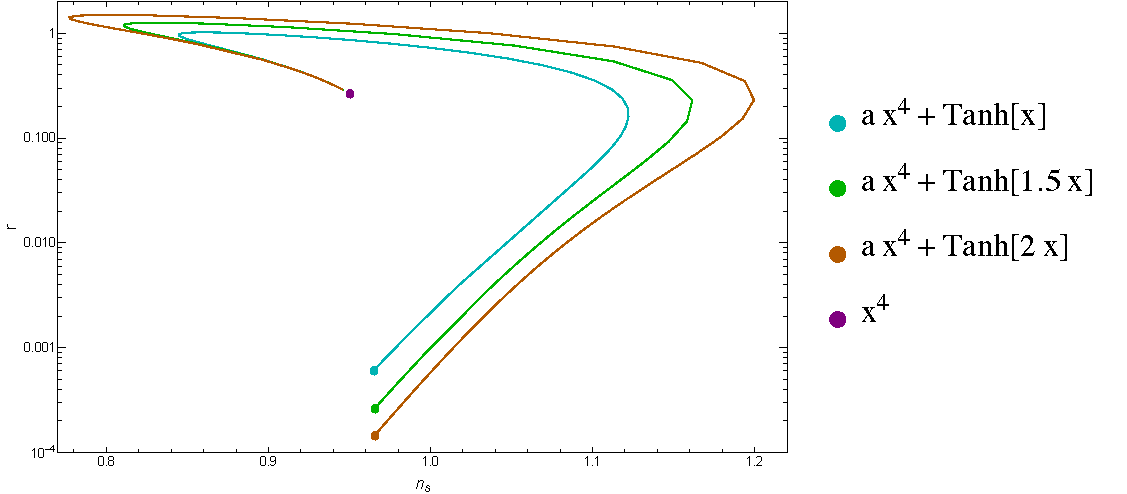
\includegraphics[width=\textwidth]{figures/LFP_lines_Tanh_final.pdf}
	\caption[Drift in \nsr plane for Tanh model with perturbations.]{A plot showing the drift in the \nsr plane as a Tanh model, $V=1+\tanh(\phi)$, is perturbed with a $\phi^4$ potential. The black circle marks the location of a pure $\phi^4$ potential, and the other colored circles mark the pure Tanh potentials.}
	\label{fig:LFP_Tanh_drift}
\end{figure}
\end{minipage}
\begin{minipage}[t][0.5\textheight][t]{\textwidth}
\begin{figure}[H]
	\centering
	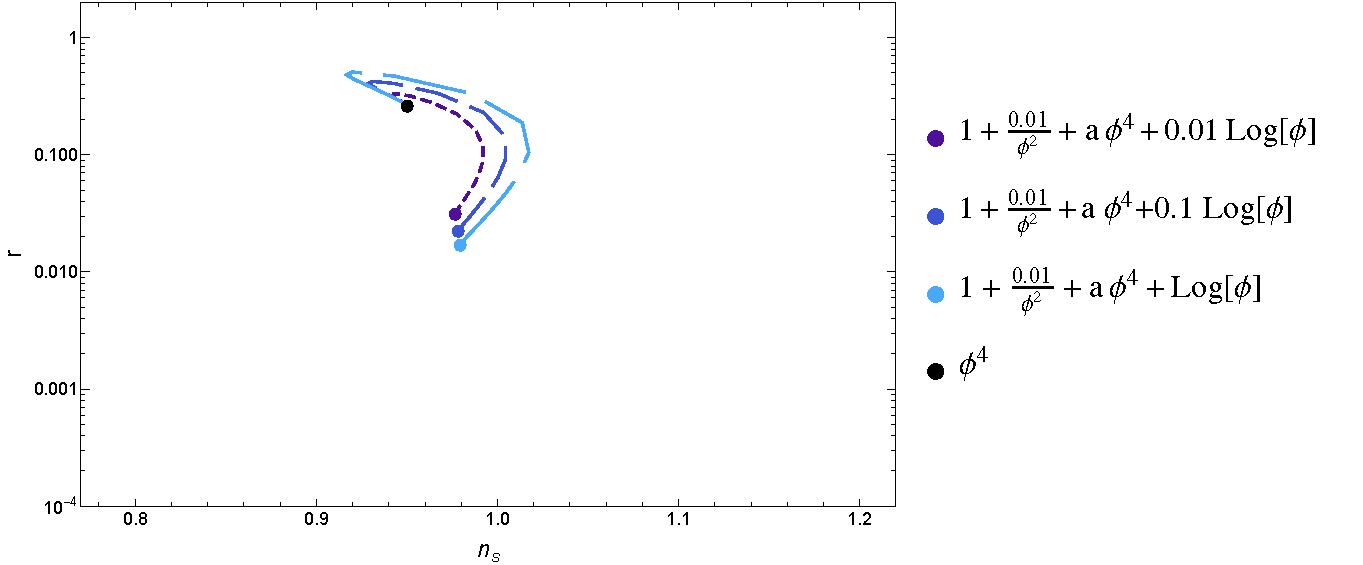
\includegraphics[width=\textwidth]{figures/LFP_lines_Log_final.pdf}
	\caption[Drift in \nsr plane for Log model with perturbations.]{A plot showing the drift in the \nsr plane as a Log model, $V=1+\tfrac{0.01}{x^2}+\log(\phi)$, is perturbed with a $\phi^4$ potential. The black circle marks the location of a pure $\phi^4$ potential, and the other colored circles mark the pure Log potentials. Note that the $\tfrac{0.01}{x^2}$ term is added to give the potential a lower bound and hence make it an acceptable model of inflation.}
	\label{fig:LFP_Log_drift}
\end{figure}
\end{minipage}
\newpage

\begin{figure}[H]
	\centering
	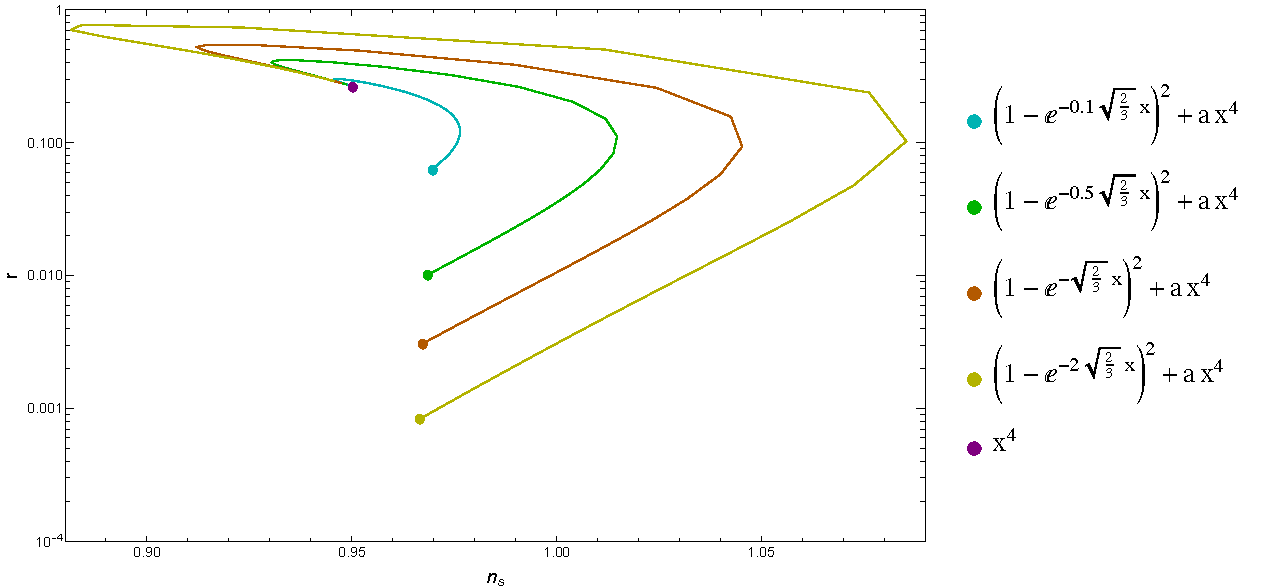
\includegraphics[width=\textwidth]{figures/LFP_lines_Rsq_final.pdf}
	\caption[Drift in \nsr plane for Starobinsky model with perturbations.]{A plot showing the drift in the \nsr plane as the Starobinsky model, $V=(1-e^{-\sqrt{2/3}\phi})^2$, is perturbed with a $\phi^4$ potential. The black circle marks the location of a pure $\phi^4$ potential, and the other colored circles mark the pure Starobinsky potentials.}
	\label{fig:LFP_Rsq_drift}
\end{figure}

Figure \ref{fig:LFP_Log_drift} shows the drift for potentials of the form $V(\phi)=1+\tfrac{0.01}{\phi^2}+a\phi^4+b\log(\phi)$. As discussed in Section \ref{ssec:LargeField}, in order to ensure that inflation ends we must force the potential to have a lower bound. We do this by adding the term $\tfrac{0.01}{\phi^2}$, which puts a minimum at $\phi=0$. Note that the curves do not drift nearly as much as they do in the Tanh model in Figure \ref{fig:LFP_Tanh_drift}. In fact, we note the trend that potentials that begin at an unperturbed \nsr point that is further from the $\phi^4$ point will drift out to larger values on the $n_s$ axis. 

This trend becomes even more apparent when we examine Figure \ref{fig:LFP_Rsq_drift}, which shows the drift in the \nsr plane due to $\phi^4$ perturbations of the Starobinsky model, $V=(1-e^{-b\sqrt{2/3}\phi})^2$. In the plot, small-dash denotes $b=0.01$, medium-dash denotes $b=0.1$, and large-dash denotes $b=1$. Again, the further the unperturbed potential is from the perturbing function, the farther it drifts when perturbed. This is concerning because \citet{Planck2015} data points to a very small value of $r$, which will push the observationally-acceptable models further from a monomial perturbing function. 

%We can quantify this effect by measuring the distance from the perturbing function and maximum amount of drift (measured from the initial, non-perturbed point). Figure \ref{fig:LFP_drift_distance} shows the maximum drift distance as a function of the initial distance from the non-perturbed point to the point corresponding to the perturbing function. The points are colored according to the model used, using the same scheme as in the previous figures: red for the Tanh models, blue for the Log models, and green for the Starobinsky models. The horizontal axis represents the initial distance from the unperturbed point (the colored circles in the drift curve figures) to the point corresponding to the perturbing function (the black circle in the drift curve figures). The vertical axis shows the drift distance, which we measure two different ways. The square points measure the distance from the unperturbed point to the point on the curve with maximum value of $n_s$. The circle points measure the distance from the unperturbed point to the point on the curve with minimum value of $n_s$. Both methods of measuring the drift distance show the same result, as would be expected from examining the drift curves of the models. We see that 
%
%\begin{figure}[h!]
%	\centering
%	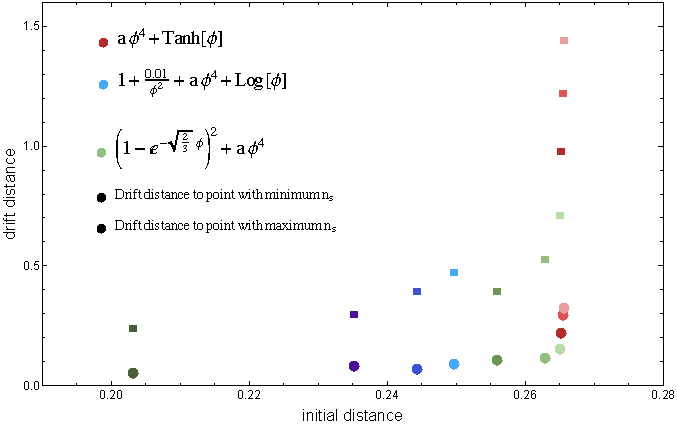
\includegraphics[width=\textwidth]{figures/LFP_drift_distance_final.pdf}
%	\caption[Drift distance vs initial distance.]{A plot showing the drift distance in the \nsr plane as a function of the initial distance from the non-perturbed point to the point of the perturbing function. The color scheme is the same as in Figures \ref{fig:LFP_Rsq_drift}, \ref{fig:LFP_Log_drift}, and \ref{fig:LFP_Tanh_drift}, with red shades denoting Tanh models, blue shades denoting Log models, and green shades denoting Starobinsky models. The horizontal axis represents the initial distance from the unperturbed point (the colored circles in the drift curve figures) to the point corresponding to the perturbing function (the black circle in the drift curve figures). The vertical axis shows the drift distance, measured two different ways, corresponding to the square and circle points. The square/circle points mark the distance from the unperturbed point to the point on the curve with maximum/minimum value of $n_s$.} 
%	\label{fig:LFP_drift_distance}
%\end{figure}

%\begin{table}[htbp]
%   \centering
%   \begin{tabular}{@{} l  c  c @{}} % Column formatting, @{} suppresses leading/trailing space
%      \toprule
%      Model & Planck Crossing ($n_s=0.977$) &  $n_s=1$ Crossing \\
%      \midrule
%      $V(\phi)=\tanh(\phi)+a\phi^4$ & $2.7\times10^{-5}$ & $8.0\times10^{-5}$ \\
%      $V(\phi)=\tanh(1.5\phi)+a\phi^4$ & $4.2\times10^{-5}$ & $1.3\times10^{-5}$ \\
%      $V(\phi)=\tanh(2\phi)+a\phi^4$ & $6.2\times10^{-5}$ & $1.9\times10^{-5}$ \\
%      \midrule
%      $V(\phi)=\log(\phi)+\tfrac{0.01}{\phi^2}+a\phi^4$ & $$ & $7.8\times10^{-5}$ \\
%      \midrule
%      $V=(1-e^{-0.1\sqrt{2/3}\phi})^2 + a\phi^4$ & $\times10^{-}$ & $\times10^{-}$ \\
%      $V=(1-e^{-0.5\sqrt{2/3}\phi})^2 + a\phi^4$ & $\times10^{-}$ & $\times10^{-}$ \\
%      $V=(1-e^{-\sqrt{2/3}\phi})^2 + a\phi^4$ & $1.0\times10^{-5}$ & $3.0\times10^{-5}$ \\
%      $V=(1-e^{-2\sqrt{2/3}\phi})^2 + a\phi^4$ & $\times10^{-}$ & $\times10^{-}$ \\
%      \bottomrule
%   \end{tabular}
%   \caption{The values of the perturbation amplitude $a$ at the point where the drift curve crosses out of the \citet{Planck2015} constraint contour and when it crosses past $n_s=1$.}
%   \label{tab:drift_crossings}
%\end{table}


\FloatBarrier
\subsection{Results for varying perturbing model}
\label{ssec:DriftVaryAf}

In sections \ref{ssec:TanhCaseStudy} and \ref{ssec:DriftResults}, we explored how perturbing the potential with a $\phi^4$ potential caused significant drift in the \nsr plane. In this section we investigate how the drift curves change as we vary the perturbing function, specifically by increasing the power of the monomial perturbation. Figure \ref{fig:LFP_Rsq_drift_af} shows a drift plot in the \nsr plane for the Starobinsky model with varying powers of perturbation. The small-dash line shows the $\phi^4$ perturbation that we explored previously. The medium-dash line shows a $\phi^6$ perturbation, and the long-dash line shows a $\phi^8$ perturbation. We only chose even powers for the perturbing functions since adding an odd-powered monomial  would make the potential unbounded and hence preclude the vacuum state necessary for the end of inflation. Notice that the $n_s$ axis had to be extended from the previous figures' scale to accommodate the $\phi^8$ perturbation's drift curve. This trend shows us that higher power perturbations induce larger amounts of drift. This is concerning since we can imagine arbitrarily large powers of perturbations and hence higher order perturbations are more likely. 

\begin{minipage}[t][0.4\textheight][t]{\textwidth}
\begin{figure}[H]
	\centering
	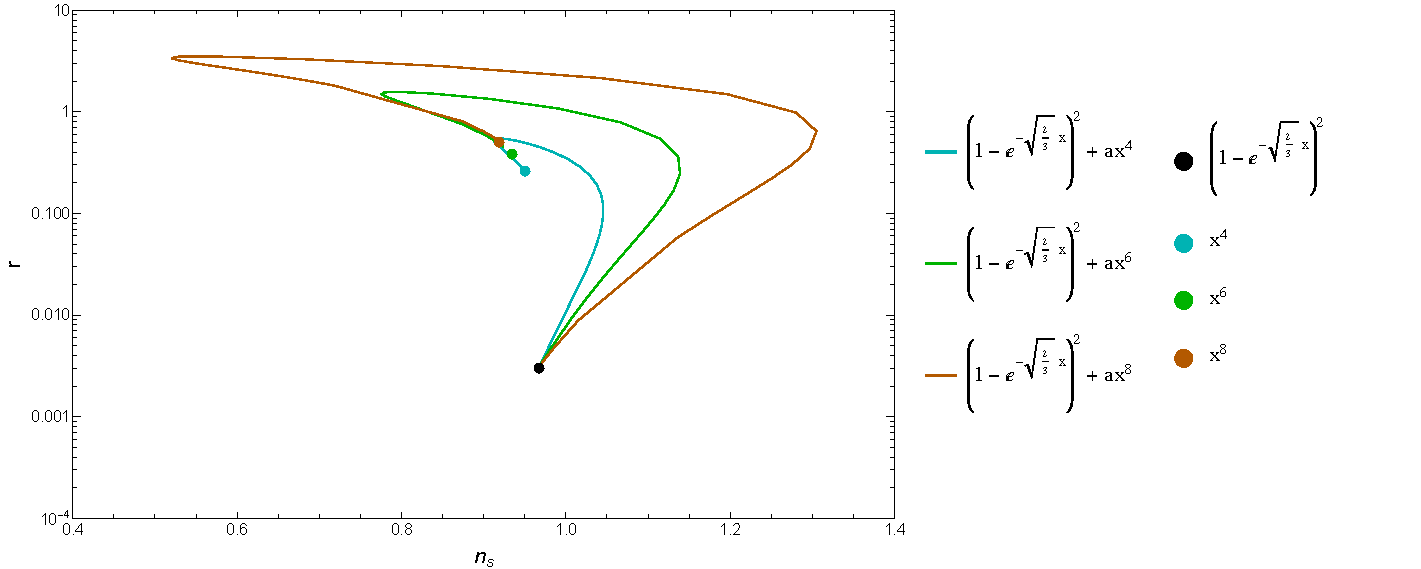
\includegraphics[width=\textwidth]{figures/LFP_lines_Rsq_varyaf_final.pdf}
	\caption[Drift in \nsr plane for Starobinsky model with perturbations.]{A plot showing the drift in the \nsr plane as the Starobinsky model, $V=(1-e^{-\sqrt{2/3}\phi})^2$, is perturbed with a $\phi^4$ potential. The black circle marks the location of a pure $\phi^4$ potential, and the other colored circles mark the pure Starobinsky potentials. The blue swatch is the \citet{Planck2015} constraint contour for the TT, TE, EE, and lowP data.}
	\label{fig:LFP_Rsq_drift_af}
\end{figure}
\end{minipage}

\begin{table}[htbp]
   \centering
   \begin{tabular}{@{} l  c  c @{}} % Column formatting, @{} suppresses leading/trailing space
      \toprule
      Model & Planck Crossing ($n_s=0.977$) &  $n_s=1$ Crossing \\
      \midrule
      $V=(1-e^{-\sqrt{2/3}\phi})^2 + a\phi^4$ & $1.0\times10^{-5}$ & $3.0\times10^{-5}$ \\
       $V=(1-e^{-\sqrt{2/3}\phi})^2 + a\phi^6$ & $1.5\times10^{-7}$ & $4.5\times10^{-7}$ \\
       $V=(1-e^{-\sqrt{2/3}\phi})^2 + a\phi^8$ & $2.7\times10^{-9}$ & $1.0\times10^{-8}$ \\
      \bottomrule
   \end{tabular}
   \caption{The values of the perturbation amplitude $a$ at the point where the drift curve crosses out of the \citet{Planck2015} constraint contour and when it crosses past $n_s=1$.}
   \label{tab:crossings_vary_af}
\end{table}

\newpage
Another way to compare the effects of the perturbation is to examine the amplitude of perturbation necessary for the curve to pass beyond the \citet{Planck2015} contours or for it to cross past $n_s=1$. Since the values of $n_s$ are so small ($<0.01$), for our purposes passing beyond the Planck contour can be approximated as passing beyond the line $n_s=0.977$. Table \ref{tab:crossings_vary_af} shows the perturbation amplitudes $a$ required to cross beyond the Planck contour and beyond the line $n_s=1$. Worryingly, by the time we get to a $\phi^8$ perturbation, it only takes a perturbation of the order $10^{-9}$ to push the potential outside of the Planck contour. This indicates that plateau models are highly sensitive to higher order perturbations. Therefore, there must be an incredible degree of fine-tuning to an infinite number of non-zero terms. 


\subsection{Results for Hilltop Models}
\label{ssec:HilltopDrift}

In order to verify that our \nsr drift method is in fact picking up the fine-tuning of the higher orders of the potential, we apply the same analysis to the polynomial hilltop models from Section \ref{sssec:Hilltop}. When we add monomial potentials $a\phi^6$ and $a\phi^8$ to a potential of the form 
\begin{equation}
V(\phi)=(\sigma^2-\phi^2)^2,
\end{equation}
we found that there was no drift whatsoever in the \nsr plane as we increased the perturbation amplitude. This is consistent with our expectations since for Hilltop models, inflation occurs at small values of $\phi$ and hence higher-order terms will be negligible. 

However, this does not mean that small field models automatically have no fine-tuning --- it merely indicates that any fine tuning in the model does not come from constraints on higher oder terms. As we discussed in Section \ref{sec:Latham}, fine-tuning in polynomial models can described via zero-counting on the equation of state, which is a more appropriate method than the \nsr drift method for the small field models. Also, since the \citet{Planck2015} results now disfavor hilltop models in favor of plateau models, it is less important that we find a means to compare the relative complexity of large and small field models. 


\FloatBarrier
%%%%%%%%%%%%%%%%%%%
%		Mukhanov	
%%%%%%%%%%%%%%%%%%%
\newpage
\section{Multiverse Problem}

In Section \ref{sec:LFP} we discussed how perturbing plateau models with large degree polynomials causes the observational results of the models to undergo a large amount of drift in the \nsr plane. We argued that this is a cause for concern because it requires us to fine-tune the potentials so that the coefficients of their series expansion have very precise, non-zero values. This method of analysis is also applicable to proposed solutions to the multiverse problem. After \citet{Planck2013} constrained $n_s$ and $r$ to values only reachable by plateau models, inflation encountered problems problems requiring smooth initial conditions and spawning a vast multiverse \citep{Ijjas+2013}. The multiverse problem can be resolved by grafting a steep slope onto the plateau \citep{Ijjas+2013,Mukhanov2014}. We show that this method of solving the multiverse problem is intractable because it encounters the same \nsr drift that we explored in Section \ref{sec:LFP}.

\subsection{Analysis of Mukhanov's model}

\citet{Mukhanov2014} proposes solving the multiverse problem by taking a plateau potential $V_p(\phi)$ and adding a singularity to produce a potential of the form:
\begin{equation}
V(\phi)=\frac{\phi_m^aV_p(\phi)}{(\phi_m-\phi)^a},
\label{eqn:MukhanovGeneral}
\end{equation}
where $\phi_m$ is the location of the singularity and $a$ is some positive power. This singularity produces a steep curve on the plateau just before $\phi_m$. To verify that this model solves the multiverse problem, we must ensure that $\phi_m$ is less than $\phi_{ei}$, the threshold for eternal inflation. In order to do so, we must first find the value of $\phi_m$ that is consistent with the observed amplitude of density fluctuations. We determine $\phi_m$ by imposing the slow roll constraints on the density perturbations:
\begin{equation}
\frac{\delta\rho}{\rho} \approx_{sr} \frac{V^{3/2}(\phi)}{V'(\phi)} \approx 10^{-4},
\end{equation}
at $\phi_{60}=\phi(N=60)$, which is in turn determined by the slow roll approximation 
\begin{equation}
\frac{V''(\phi_N)}{V(\phi_N)} \approx_{sr} \frac{1}{N}
\end{equation}
\citep{MukhanovBook2005}. Once we have found $\phi_m$, we At values of $\phi$ greater than $\phi_{ei}$, the universe would undergo eternal inflation do to self reproduction, in which quantum fluctuations are large enough to spawn an infinite number of causally disconnected universes. This is a problem because this produces an infinite number of universes with varying laws of low energy physics \citep{Linde2008,Linde1986}. Since in an infinite multiverse every possible universe will occur and will do so an infinite number of times, a self reproducing theory loses all of its predictive power. Grafting a steep slope onto the plateau solves this problem by \mep{Insert explanation here}. 

As an example, \citet{Mukhanov2014} takes a potential of the form
\begin{equation}
V(\phi)=\frac{(1-e^{-\phi})^2}{(\phi_m-\phi)^4}
\label{eqn:MukhanovExp}
\end{equation}
and claims that it is ``perfect agreement with observations''. However, we find that this is only true for very large values of $\phi_m$ and that once $\phi_m$ is made small enough to counter eternal inflation, the potential no longer lies within the \citet{Planck2015} contours. 

\begin{figure}[h!]
	\centering
	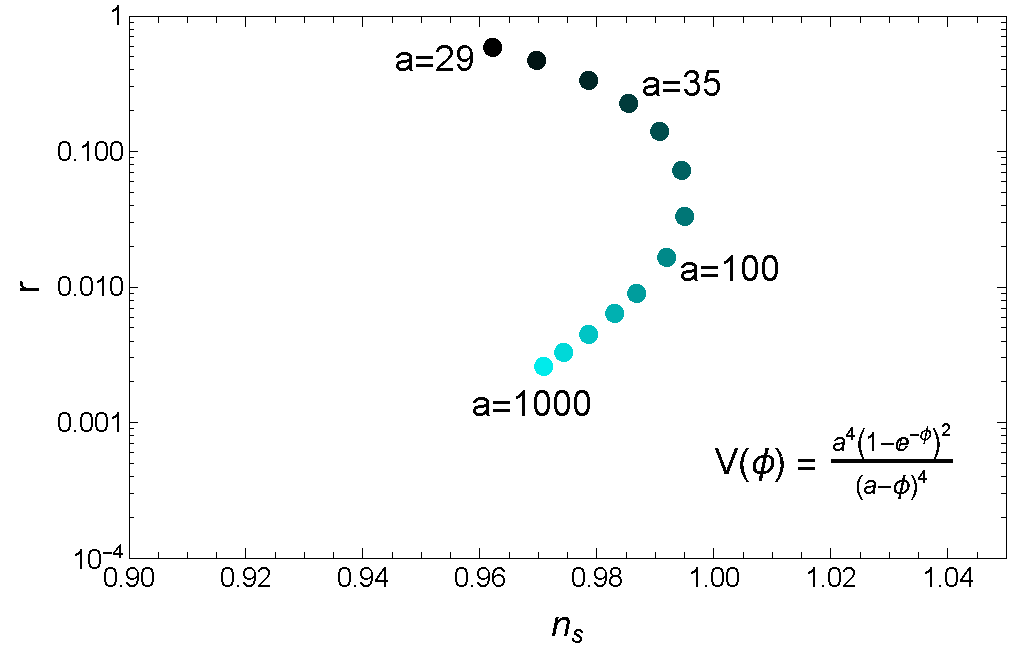
\includegraphics[width=\textwidth]{figures/Mukhanov.pdf}
	\caption[Drift in \nsr plane for Mukhanov model as the singularity moves to smaller $\phi$.]{A plot showing the drift in the \nsr plane as the singularity $\phi=\phi_m$ in the Mukhanov model, $V=\tfrac{(1-e^{-\phi})^2}{(\phi_m-\phi)^4}$, is moved to smaller values of $\phi_m$ (i.e. closer to the 60 efold mark). The coloring of the markers corresponds to the value of $\phi_m$, with darker shades indicating smaller $\phi_m$. The blue swatches are the \citet{Planck2015} constraint contours used previously.}
	\label{fig:Mukhanov_drift}
\end{figure}

Figure \ref{fig:Mukhanov_drift} shows an \nsr drift plot similar to those discussed in Section \ref{sec:LFP}, but using Equation \ref{eqn:MukhanovExp} for the potential and varying $\phi_m$ instead of the perturbation amplitude. For very large values of $\phi_m$, $\phi_m=1000$, the potential remains within the \citet{Planck2015} contour. However, by the time $\phi_m=300$ (still a quite large value!), the potential's \nsr value has moved outside the constraint contour. This is very problematic in terms of fine tuning because it shows that in order to have preserve observational results, the steep slope must be pushed back to very large values of $\phi$. 

\citet{Mukhanov2014} calculated the value of $\phi_{ei}$ to be $1000$ for the potential in equation \ref{eqn:MukhanovExp}. Therefore, in this specific case it turns out that the observational results are achievable for $\phi_m$ very close to $\phi_{ei}$. However, \citet{Mukhanov2014} also suggested a model with the potential
\begin{equation}
V(\phi)=\frac{(1-e^{-\phi})^2}{(\phi_m-\phi)^6},
\label{eqn:MukhanovExp6}
\end{equation}
where the singularity has order 6 instead of 4, giving the barrier a steeper slope. When we perform the \nsr drift analysis on this model, we obtain the results presented in Figure \ref{fig:Mukhanov6_drift}. Recall from Section \ref{ssec:DriftVaryAf} that increasing the power of the perturbing monomial increased the amount of drift and also increased the sensitivity to the perturbation amplitude. We see the same behavior with Mukhanov's model, where increasing the order of the singularity increases the amount of drift in the \nsr plane. We also notice that singularities at higher values of $\phi_m$ produce the same amount of drift as smaller values of $\phi_m$ did for the 4th order singularity. While in the 4th order case the model did not drift out of the \citet{Planck2015} constraint contour until around $\phi_m=300$, in the 6th order case the model drifts out of the contour by $\phi_m=500$. For comparison, $\phi_{60}$ is about 5 for these models. 

This sensitivity is particularly worrying, not just because a barrier at such a large value as such dramatic observational effects, but also because \citet{Mukhanov2014} calculated $\phi_{ei}$ to be 100 for the 6th order model. In order to prevent eternal inflation and the multiverse problem, Mukhanov proposed inserting the singularity as a barrier to prevent the field from accessing values in the eternally-inflating regime. Therefore, for the potential to avoid the multiverse problem, it must have $\phi_m<\phi_{ei}$. However, for the 6th order singularity, we find that using a value of $\phi_m<\phi_{ei}\approx100$ will cause an unacceptable amount of \nsr drift. Therefore, Mukhanov's proposed method of avoiding the infinite multiverse is at best finely-tuned and at worst inconsistent with observations. 

\begin{figure}[h!]
	\centering
	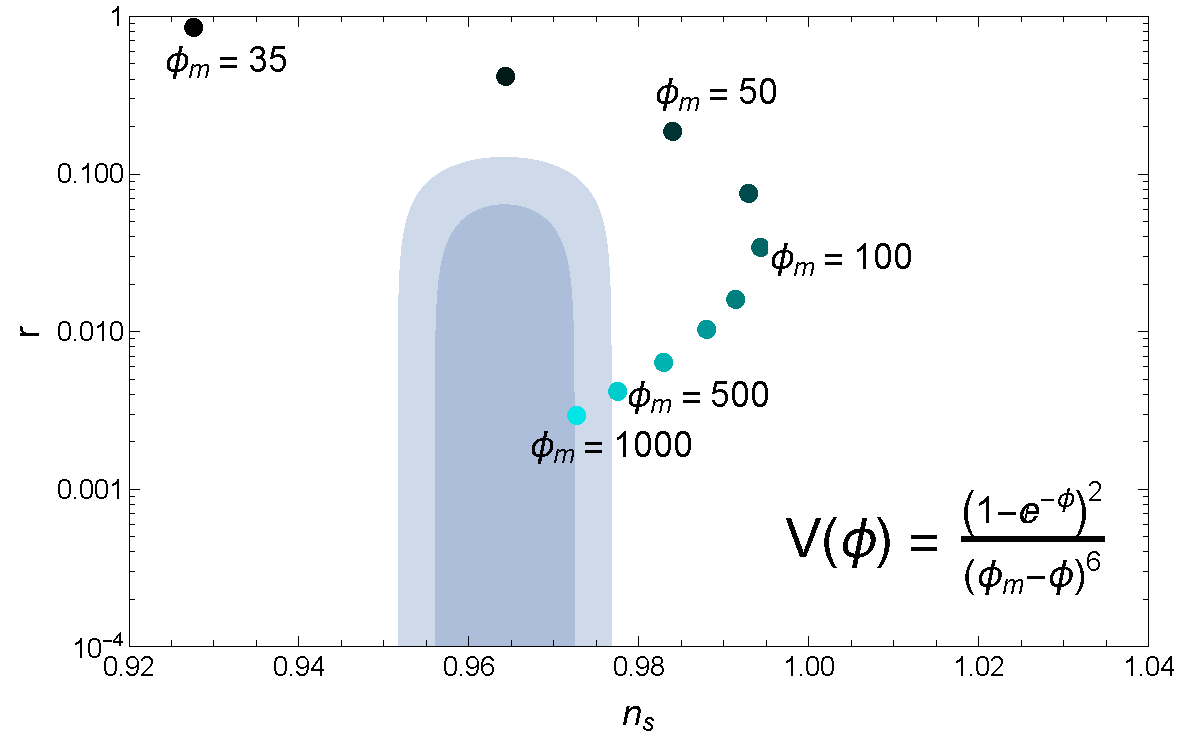
\includegraphics[width=\textwidth]{figures/Mukhanov6.pdf}
	\caption[Drift in \nsr plane for Mukhanov model as the singularity moves to smaller $\phi$.]{A plot showing the drift in the \nsr plane as the singularity $\phi=\phi_m$ in the Mukhanov model, $V=\tfrac{(1-e^{-\phi})^2}{(\phi_m-\phi)^6}$, is moved to smaller values of $\phi_m$ (i.e. closer to the 60 efold mark). The coloring of the markers corresponds to the value of $\phi_m$, with darker shades indicating smaller $\phi_m$. The blue swatches are the \citet{Planck2015} constraint contours used previously.}
	\label{fig:Mukhanov6_drift}
\end{figure}

\subsection{Analysis of other similar models}

\FloatBarrier
%%%%%%%%%%%%%%%%%%%
%		Conclusions	
%%%%%%%%%%%%%%%%%%%
\newpage
\section{Conclusions}

The field of inflationary cosmology comes with such grand successes that it is often hard to also see its shortcomings, even ones potentially grievous. As a theory, inflation is extremely attractive because it solves many perplexing problems, namely the horizon, flatness, and monopole problems, that otherwise do not have any clear solution. Although at first the idea of inflationary theory seems simple and elegant --- all we do is add to the Standard Model a scalar field with an appropriate potential and we get an inflating universe --- as the field has developed the form of the potential has been constrained more and more by both theory and observation. Observations of the CMB have constrained both the spectral tilt and tensor-to-scalar ratio of the density perturbations of the early universe to incredible precision, and these results are not consistent with the most obviously simple inflationary potentials, such as $\phi^2$, $\phi^4$, and other monomial or low-order polynomials. On the theory side, cosmologists have developed constraints such as the slow roll conditions to solve the graceful exit problem. The theory has recently encountered a new problem, that of eternal inflation and the inflationary multiverse. This problem constrains inflation to models that cannot reach a threshold $\phi_{ei}$, after which quantum fluctuations dominate the evolution of the field and hence prevent the end of inflation. In the face of all of these constraints, inflationary models have increased in complexity to the point where some have called into question the validity of the field itself.

My thesis works to take these vague notions of complexity and fine-tuning and define specific measures for determining the degree of fine-tuning in an inflationary model. Our work builds off of the work of \citet{Boyle+2006}, who uses the evolution of the equation of state to determine the degree of fine-tuning in an inflationary potential. Specifically, the degree of fine-tuning is defined to be the number of zeros in the equation of state and its derivatives. We examine Boyle's results in light of the recent \citet{Planck2015} observational constraints, which together show that the simplest models by Boyle's measure are the least consistent with current observations. 

Boyle's method works well for the polynomial models considered in the paper; however, the recent Planck results have favored a new class of models: plateau potentials. The main part of my project explored a new method of examining the fine tuning in plateau models, using perturbation by a monomial term in the potential. The motivation for this method stems from the idea that plateau models are fine-tuned because the series expansion of their potentials contain an infinite number of non-zero terms that must be precisely balanced to create a plateau. We investigate this general intuition by taking a plateau potential and perturbing it with a monomial term such as $a\phi^4$. We then track how increasing the perturbation amplitude $a$ affects the observational parameters $n_s$ and $r$. We find that increasing $a$ causes significant drift in the \nsr plane, until with a large enough perturbation amplitude it converges on the \nsr values for the perturbing function. 

This methodology provides two means of quantifying the degree of fine tuning: either by measuring the amount of drift in $n_s$ and $r$ or by measuring the the amplitude of perturbation required for a certain amount of drift (e.g. to drift out of the Planck contours or to drift past $n_s=1$). We find that the Tanh models have the largest total drift in the \nsr plane, while the \mep{BLANK} models are the most sensitive to the perturbation amplitude. We also investigated how the power of perturbing function affected the total drift and sensitivity, finding that the higher order monomials induced larger net drift and greater sensitivity to the amplitude of perturbation. These results are especially concerning for plateau models because it tells us that the higher order terms are extremely sensitive to perturbation and must be very finely balanced in order to reproduce observations. This sensitivity is a significant manifestation of fine-tuning in plateau potentials and merits the attention of theorists as they design such models.

The sensitivity of plateau models to high-order perturbations has definite theoretical consequences. Adding a monomial perturbation has the effect of grafting a steep slope onto the plateau. However, \citet{Mukhanov2014} used exactly this idea to propose a solution to the multiverse problem. In order to make the eternally-inflating regime $\phi>\phi_{ei}$ inaccessible, Mukhanov inserted a singularity in his potential at $\phi_m<\phi_{ei}$, effectively grafting onto the plateau a steep slope asymptoting to $\phi=\phi_m$. We applied our \nsr drift methodology to Mukhanov's model, tracking how the observational predictions changed as we decreased $\phi_m$ (and hence brought the slope closer to the edge of the plateau and the $\phi_{60}$ mark). We found that bringing the singularity only as close as $\phi_m=300$ (for reference, $\phi_{60}\sim5$) causes a drift large enough for the potential to leave the Planck contours. Although Mukhanov's 4th order singularity model is allowed $\phi_m$ as large as 1000 and hence can remain within the Planck contours, the 6th order singularity model is only allowed $\phi_m\lesssim100$, which takes the predictions far outside the Planck constraints. Thus, Mukhanov's proposed solution is on shaky grounds. 

\newpage
In conclusion, we find that considering the predictive consequences of perturbations is a productive way to measure the fine-tuning in plateau potentials. The large amount of drift caused by tiny perturbation amplitudes is a significant concern when it comes to constraining large field plateau models. As theorists continue to construct new models of inflation, it will be important to keep in mind the instabilities inherent in plateau potentials. If this and other manifestations of fine-tuning continue to plague inflationary theory, it might even be advisable to extend one's outlook to other theories of the early universe, such as ekpyrotic or cyclic models, that might be able to solve the horizon, flatness, and monopole problems without resorting to finely-tuned models. Further work in exploring the existence/amount fine-tuning in such non-inflationary theories is recommended to compliment the work done on the subject within inflationary theory. 

%%%%%%%%%%%%%%%%%%%
%		Appendix	
%%%%%%%%%%%%%%%%%%%


\newpage
\bibliographystyle{apj}
\bibliography{thesis}

\end{document}
